\documentclass{uscthesis}

%%%%%%%%%%%%%%%%%%%%%%%%%%%%%%%%%%%%%%%%%%
%%% Options include: [forbinding], which produces 
%%% an alternative title page and an appropriate
%%% binding margin, and [honors] for Honors College theses.
%%%%%%%%%%%%%%%%%%%%%%%%%%%%%%%%%%%%%%%%%%

%%%%%%%%%%%%%%%%%%%%%%%%%%%%%%%%%%%%%%%%%%
%%  LaTeX Preamble
%%%%%%%%%%%%%%%%%%%%%%%%%%%%%%%%%%%%%%%%%%

\usepackage{graphicx}
%\usepackage{tikz}
\usepackage{pstricks,pst-node,pst-plot}
\usepackage{stmaryrd}
\usepackage{enumerate, multirow}
\usepackage{pdfpages, pdflscape}
\usepackage{appendix}
\usepackage{url}
%\usepackage{caption}
%\usepackage[dvipdfmx]{graphicx} 

%%%%%%%%%%%%%%%%%%%%%%%%%%%%%%%%%%%%%%%%%%
%% The packages above are only examples. You should include 
%% any LaTeX packages that you need.  Most packages should work 
%% with this documentclass. If you do not use the 
%% packages in the example above, don't put these
%% lines in your file.
%%%%%%%%%%%%%%%%%%%%%%%%%%%%%%%%%%%%%%%%%

\bibliographystyle{amsplain}

%%%%%%%%%%%%%%%%%%%%%%%%%%%%%%%%%%%%%%%%
%% The line above specify a BibTeX style which controls 
%% the appearance of the bibliography and how citations to
%% the bibliography within the text will work.  Other options beside 
%% amsplain are available. For instance
%%
%% \bibliographystyle{plain}
%%
%% which resembles amsplain but is less elaborate. 
%%
%% You could replace the line above by the following three lines
%%
%% \usepackage{natbib}
%% \bibliographystyle{plainnat}
%% \usepackage{uscnatbib}
%%
%% to get an author-date system recommended by the Chicago 
%% Manual of Style. You have to get the package uscnatbib.sty 
%% from the Graduate School.
%%
%% A second possibility is to replace the line above by
%%
%% \usepackage[style=uscnumeric]{biblatex}
%% \bibliography{\jobname}
%%
%% or by
%%
%% \usepackage[style=uscauthoryear]{biblatex}
%% \bibliography{\jobname}
%%
%% The first of these two alternatives is like \bibliographystyle{plain}
%% while the second produces an author-date sytem recommended by the 
%% Chicago Manual of Style.  You have to download the supporting files
%%
%% uscnumeric.bbx
%% uscnumeric.cbx
%%
%%    or
%%
%% uscauthoryear.bbx
%% uscauthoryear.cbx
%%
%% from the Graduate School.
%%
%% These two options use the biblatex.sty package, which is included with 
%% most up-to-date LaTeX installations.  This package provides a powerful
%% an flexible alternative to the traditional way BibTeX has been used.
%% 
%% A third possibility is to use the amsrefs package,  an 
%% very attractive alternative to BibTeX. To use this possibility
%% replace the \bibliographystyle{amsplain} with the following lines 
%%
%% \usepackage{uscamsrefs}
%%
%%     or
%%
%% \usepackage[author-year]{uscamsrefs}
%%
%% The first alternative produces a bibliography like that produced
%% by \bibliographystyle{amsplain} while the second produces an author-date
%% system recommended by the Chicago Manual of Style. To use this option
%% you have to download the file 
%% 
%% uscamsref.sty
%%
%% from the Graduate School.
%%
%% The three systems suggested above that to conform the Chicago Manual of Style
%% provide several different commands for you to use in the text when
%% citing an item in your bibliography.  The three systems do this job
%% differently.
%%
%% 
%%In any case, this  is a good spot to ask LaTeX to load what it needs to handle
%% literature citations and to layout the bibliography. 
%%
%%%%%%%%%%%%%%%%%%%%%%%%%%%%%%%%%%%%%%%%%%

%\newcommand{\join}{\vee}
%\newcommand{\meet}{\wedge}
%\newcommand{\w}{\omega}
%\newtheorem{thm}{Theorem}[chapter]
%\newtheorem*{thmun}{Theorem}
%\newtheorem{cor}[thm]{Corollary}
%\newtheorem{lem}[thm]{Lemma}
%\theoremstyle{definition}
%\newtheorem{defn}[thm]{Definition}
%\newtheorem{ex}[thm]{Example}
%\theoremstyle{plain}

%%%%%%%%%%%%%%%%%%%%%%%%%%%%%%%%%%%%%%%%%%%%
%%  Again, this is just a few sample lines. Put here any 
%%  commands of your own devising that you want to use.
%%  If these examples are no use to you, omit them.
%%%%%%%%%%%%%%%%%%%%%%%%%%%%%%%%%%%%%%%%%%%%%


%%%%%%%%%%%%%%%%%%%%%%%%%%%%%%%%%%%%%%%%%%%%%%%%%%%%%%
%%             The Front Matter
%%  The section below deals with the material that comes 
%%  before the actual content of the document: The title 
%%  page, abstract, acknowledgments,etc.
%%
%%  Some of it is required.
%%%%%%%%%%%%%%%%%%%%%%%%%%%%%%%%%%%%%%%%%%%%%%%%%%%%%%

\title{A Multiagent Approach Towards Solving Complex Problems of Sociotechnical Systems}

\author{Hongying}{Du}    %% First Name then 
                                 %% Last Name

\date{2014}                      %% The year of graduation

%\month{December}                 %% Only for the honors option
                                 %% where it is REQUIRED

\otherdegrees{
Bachelor of Engineering\\
Northwestern Polytechnical University 2006\\ [3pt]
Master of Engineering\\
Northwestern Polytechnical University 2009\\ %% The \\ on this line is 
}                                %% ESSENTIAL!

\degree{Doctor of Philosphy}     %% The Graduate School provides 
                                 %% a list of official degrees.
\field{Computer Science and Engineering}              %% Fields also provided by the 
                                 %% Graduate School.
\college{College of Engineering and Computing}  %%As listed by Grad School

\advisor {Dr.}{Michael N. Huhns}{Major Professor}  %%% Be sure the 
\readera{Dr.}{Manton M. Matthews}{Committee Member}     %%% third field is 
\readerb{Dr.}{Jos{\'e} M. Vidal}{Committee Member}          %%% the one used in 
\readerc{Dr.}{Munindar P. Singh}{External Examiner} %%% your department.
\readerd{Dr.}{Kuldar Taveter}{External Examiner}	
%%% If you have just two readers, for example, leave out \readerc and
%%% \readerd
%%%
%%% For Honors College theses use \reader{}{}   NO third field.
%%% The commands \otherdegrees, \degree, \field, \college, \readera, etc.
%%% are not used under the honors option.
%%%%%%%%%%%%%%%%%%%%%%%%%%%%%%%%%%%%%%%%%%%%%%%%%%%%%%%

\dean{Lacy Ford}   %% The Dean of the Graduate School
                     %% For Honors College theses use
                     %% \schcsigner{}{}.  For example,
                     %% \schcsigner{Dr.}{Davis Baird}

%me \copyrightpage       %% This is optional. It makes a 
                     %% copyright page that will appear 
                     %% immediately after the title page.

\abstract{abstract/abs}  %% This calls the file herkimer.tex but 
                     %% but you might replace herkimer by 
                     %% anything you like, for example by 
                     %% abstract. Note, the Graduate School
                     %% REQUIRES that PhD dissertations have 
                     %% abstracts.
                     %%
                     %% For Honors College theses use
                     %% \honorsabstract{}

%\summary{precis}     %% This command calls  precis.tex
                     %% It is only available with the honors
                     %% option and it is REQUIRED for Honors
                     %% theses. 

\acknowledgments{acknowledge/ack} %% This calls the file thanks.tex 
%% This is optional       %% where you have put your 
                          %%acknowledgments.

%\dedication{dedication}   %% Calls dedication.tex
%%% Also optional

%\preface{forward}    %% Calls forward.tex.  Optional.

\makeLoT               %% Issue this command if your work has 
                       %% four or more tables.  A list of tables 
                       %% will be produced automatically.

\makeLoF               %% works the same way but for figures.

%%%%%%%%%%%%%%%%%%%%%%%%%%%%%%%%%%%%%%%%%%%%%%%%%%%%%%%%%%%%
%%  Finally, here is the meat.  The idea is to compose a 
%%  .tex file for each section of your thesis or dissertation.  
%%  Then use LaTeX's \include command to put them all together.  
%%  Doing it this way makes it easier to change the order of 
%%  exposition as your writing is in progress.  Also it
%%  makes it easy to print out just one section. The \include
%%  command always starts a new page. So every section would 
%%  start on a new page.  If you would like for sections just
%%  to continue, after the appropriate vertical space, on the
%%  current page, then use the \input command instead of the 
%%  \include command.
%%%%%%%%%%%%%%%%%%%%%%%%%%%%%%%%%%%%%%%%%%%%%%%%%%%%%%%%%%%%

\begin{document}

% ********** Chapter 1 **********
\chapter{Introduction}
\label{ch0}

As the amount of communication among people increases rapidly and the technology grows fast, more complex problems occurs and humans don't have enough time, energy, or ability to tackle with all these problems. Our work involves one complex problem -- scarce resource allocation problem. To help humans with these problems in sociotechnical systems, we took advantage of multiagent systems in which autonomous agents represent humans' interests and make decisions for humans. 

In implementing such systems, we need to handle two technical issues. First, how the agents represent humans and how the agents interact with each other in the systems. Second, how we represent the interaction between humans and agents. Our work contains three study cases, while the first two cases, shopping route optimization and health care provider selection through recommendations investigate the first issue. The third case is about human-agent interaction while playing a game, which explores the second technical issue. 

This introduction continues with more detailed explanation for the purpose of study in section \ref{ch0:PurposeOfStu} and a description of complex problems and possible solutions in section \ref{ch0:problemsAndSol}. To find solutions for these problems, we need some technical help from the artificial intelligence domain. In section \ref{ch0:MotivatingExa}, we explain what motivates our study cases in this work.

\section{Purpose of Study}
\label{ch0:PurposeOfStu}

Because human societies are complex and humans rely on resources that are scarce, we encounter complex resource allocation problems. Scarce resources might be different under different circumstances, such as food, energy, medical care, clean water, etc. To solve these problems, human interact with each other, and the interaction or information flow among them forms different kinds of information systems. Together with the technical aspects that participate in the systems to help, the information systems are actually sociotechnical systems, as we will define later. There are various kinds of sociotechnical systems serving different purposes. Take a simple situation as an example, a patient is trying to find a doctor who could take care of him. He may have a goal to spend money as less as possible, or to cure him as soon as possible, but he has no idea which doctor fits his purpose best. Thus he turns to his friends, his friends' friends if necessary, for recommendations, incorporate these information into consideration, and make a decision with the help of agents. In this example, the persons involved, the agents and the information flow form a sociotechnical system and the purpose is to find a doctor for the patient. There are more complex information systems like the ones in section \ref{ch0:problemsAndSol}. 

As the scale of a system grows, more complex problems, some with global interactions which lead to global consequences, emerge. In many cases it is hard to find solutions to the problems or perform experiments on real systems due to various reasons, such as difficulty of synchronization, long time span of doing the experiments, or extreme geological conditions.

Because of complexity of the systems, the huge amount of information flow and other factors that make the problems hard to solve, humans need computational help in designing, implementing, and evaluating the systems. With the technical help of simulated systems, the cost of experiments is reduced and the purpose of study is fulfilled. Several questions need to be considered while designing a simulated sociotechnical system. For instance, how big should the system be and what entities are involved? What kind of information should be kept an eye on? What consequences to expect and what goals to achieve? We'll see more analysis in system design in section \ref{ch0:problemsAndSol}. 

Humans involved in complex problems usually only have access to partial information and they try to achieve a common goal while pursuing their own interests. This characteristic is consistent with the feature of distributed systems where agents with partial information are used to assist humans to make decisions. Such systems with multiple agents are called MultiAgent Systems (MAS). Agents are an autonomous software entities that can act on the behalf of his principle, sometimes a human in a sociotechnical system, based on his knowledge and judgment. This natural characteristic makes an agent a good representative of a human. Also, the amount of information flow in a sociotechnical system could be potentially enormous, which is beyond the processing ability of humans brain, thus it is better to have an autonomous agent gather information, communicate with other agents and make decisions on behalf of a person. A multiagent system is a system/society that gathers multiple agents who interact with each other. Information is exchanged among the agents who have goals based on their principles' interests. Nowadays agent technology is used everywhere, ranging from industry such as fault detection, energy distribution, to everyday life, such as web services, security patrols. First two case studies in this dissertation use multiagent systems to implement a grocery shopping scenario and a health care system.

Due to the popularity of the agents existed in our society it is inevitable that human-agent mixed societies emerge. In such societies, humans and agents exchange information and work together to achieve a particular goal, compete with each other, or have more complex relationships. Examples of working together include teaching children languages or mathematics using emotional agents. An emotional agent is an agent with emotions which are expressed by expressions of its animated face on the screen, words programmed in it, and so on. If a child answers a question correctly or performs well, the agent smiles or does other positive expressions and actions. An example of competition is that humans and agents take part in an auction and bid for some goods on the Internet. 

It is important to understand how humans and agents interact in various human-agent mixed societies in different aspects. For example, will humans have the same performance in the mixed societies as previous while there's no agent involved? What factors influence humans' decisions/attitude towards agents? Do humans' personalities play a part in their decisions and how? Many researchers studied the first two questions but less studied the third question. The third part of this dissertation is trying to get an insight into the questions about relationship between personalities and decisions. Conclusions to these questions could be used in many ways. For example, we could predict the performance of humans in a game knowing their personalities, or assign an agent with the "proper" personality to accompany a human, etc.     

\section{Complex Problems and Possible Solutions}
\label{ch0:problemsAndSol}

The problems human encounter everyday range from very personal, such as what to eat for breakfast, to very influential, such as what the best plan is for a company. Nowadays problems become more and more complicated, considering the following three factors:
\begin{itemize}
\item[-]size: since the communication of people and exchange of information are very frequent today due to the development of new technologies and market needs, it is very possible that problems encountered have larger size than ever before. For example, people like to take digital pictures and put it on the Internet, and with the increasing size of digital photos today, it takes a lot of space to store these photos and more time to find specific photos. Another example is integrating several databases of huge amount of data. Because the databases are huge and there are complex relationships among them, any operation should be considered or evaluated before they are actually performed. The size of a problem matters because it could motivate new technologies which deal with new challenges brought by the size.
\item[-]intersection: a problem may involve different areas and intersect or overlap with other problem domains. For example, consider the problem of arranging the routes of goods transportation of a delivery company everyday. First a couple of key time points should be considered, such as the arrival time of goods to the company. Other things to be considered include available transportation vehicles and human labors, weather, and so on. This problem involves human resources, scheduling, in addition with the help of weather forecasting, and some other areas. For complex problems, it is inevitable that they involve different areas and it is beyond the capacity of just humans, which is why we need the help of technology.     
\item[-]consequences: due to the above two factors and globalization, some problems today have more influential consequences than before. For example, an erroneous operation on databases of a large electricity company may lead to failure of several power plants, causing residents of an area short of electricity. Another example is global warming, which caused by multiple reasons. Possible reasons include increasing size of people and cars therefore more carbon dioxide, decreasing area of forests, polluted air and seas, and so on, which are all interrelated that the problem couldn't be solved with the effort of only a portion of people. Some events, such as nuclear disaster, happen on one location of the world, but continuously have global consequences, such as the release of radioactive materials.              
\end{itemize}

Because of these factors, some problems are so complex that technical help designed to deal with the complexity of these problems is needed. There are two parts or aspects of the technical help: 
\begin{itemize}
\item[-]How a technical system represents each person and their interactions with each other and the problem domain. For example, we need to decide how the agents communicates in a multiagent system under a particular situation.
\item[-]How a person interacts with the system. For example, we could have a person specify his preferences by selecting some options on a web page.
\end{itemize}
Since multiagent systems represent the feature of complex problems well in the sense that information centralization isn't a must in the systems and that autonomous agents could represent persons well, multiagent systems are used in this work.

\section{Research Methodology}
\label{ch0:MotivatingExa}
For the various complex problems existed in the sociotechnical systems everywhere nowadays, humans don't have time or interests to work with other humans on these problems, so humans need agents to represent them which could relieve them from tasks or pressure. Therefore, we turned to multiagent systems for technical help. 

As for research methodology, which should depend on the research questions, we uses case study approach to investigate the aspects of implementing a sociotechnical system in depth. As Yin \cite{yin2009} said, case study is "an empirical inquiry about a contemporary phenomenon (e.g., a "case"), set within its real-world context-especially when the boundaries between phenomenon and context are not clearly evident." Case study could be used if the research addresses a descriptive question or an explanatory question, such as "What is happening?", or "Why or how is it happening?" \cite{shavelson2003}, which is exactly what we need. 

In this work, we studied three cases. First, can you imagine an agent would help you to list the goods that you want to buy just by scanning the barcode of your goods that's running out or taking pictures of them, calculate the optimal route based on your location and your preferences such as which stores you usually visit, and provide suggestions? In the first case study, we try to find the optimal route for a customer who wants to do shopping. First we rely on a multiagent system to publish and retrieve information related to the items sold in store, such as price and quality. Then an agent representing the customer will provide a solution for the customer according to the shopping list by giving suggestions of which stores to visit. We used simulated data and real-world data to test our approach and then evaluated the robustness of the system.

Second, have you ever troubled by the question of which physician or doctor to visit when you are ill? How would you know whom is good for you, especially if you don't have experience with any of them? Of course you could search online, but the information there may be misleading and outdated. In our healthcare system, an agent representing you could interact with the agents of your friends, or even your friends' friends, to acquire information, integrate them, and make a suggestion based on your preference, such as saving money, or heal fast. Friends' agents have their choices of whether to respond to the patient's agent or not. In this case, we investigate the interaction among agents.  

Third, do you like or fear to interact with agents? Have you wondered what factors influence your emotion or affection towards agents? These questions are encountered inevitably while designing a multiagent system. In our last case, we studied the effect of a particular factor - personality - on the decisions humans made while interacting with agents and other humans in a mixed human-agent society. Human subjects were guided to play a variant of cake-cutting game and then asked a question of how they would like to divide the leftover cake between the simulated human and the agent participated in the game. So the questions are, would personality play a part in humans' decisions and is there any pattern for the answers to the question?

The three cases come from different domains and it seems that they are unrelated, but actually not. In the shopping scenario, agents contributed data to a central server and receive data from a central server, so the agents interacted indirectly, but a customer's shopping agent and other persons' shopping agents might not talk to each other. In the healthcare case, agents work with or interact directly with other agents on the problem. In the human-agent interaction case, we investigate how a person would interact with his agent, and how an agent would interact with a person and with other agents. Therefore, the first two cases studied the first aspect of the technical help and the third case investigated the second aspect. The three cases contribute to what we need for implementing a simulated sociotechnical system. 
  
% ********** End of chapter **********

% ********** Chapter 1 **********
\chapter{Background}
\label{ch1}

Before implementing a sociotechnical system, we need to understand what a sociotechnical system is and its characteristics, problems in the system and possible solutions of the problems. Whitworth and Ahmad \cite{whitworth2013} claimed a sociotechnical system as a social system operating on a technical base, such as email, chat, Facebook, and described the design process of a sociotechnical system. Why do we need a sociotechnical system instead of a common computer-based or technical system? As Baxter and Sommerville \cite{baxter2011} stated, systems often meet their technical "requirements" but are considered to be a "failure" because they do not deliver the expected support for the real work in the organization. The source of the problem is that techno-centric approaches to systems design do not properly consider the complex relationships between the organization, the people enacting business processes and the system that supports these processes.

In this chapter, first we present background knowledge of sociotechnical systems, including the concept and some keywords related to our work. Then we introduce a complex problem of sociotechnical systems that is related to our case studies here - the resource allocation problem. At last, multiagent systems are introduced to tackle the problems in a sociotechnical system.  

\section{Sociotechnical Systems}
\label{ch1:sociotechnicalSys}
For solving complex problems, we should understand the environment that the problems build on, i.e., different kinds of sociotechnical systems. Today everyone lives in some sociotechnical systems one way or another. The name "SocioTechnical Systems" indicates both the social aspects, such as humans or society, and the technical aspects, such as organizational rules and policies in the system. Through interaction and cooperation of all the participants in the system, it is expected to achieve solutions better than that achieved with only technology or humans available in the system. Let's consider some examples on top of the find-a-doctor example mentioned before. 

Sociotechnical systems are common and play an important role in our era due to increasingly complex societies, which rely on increased connectivity and global interactions between humans and technology. Information globalization changes human life in many ways, from communication between friends, to the way the companies operate their business. All these require the cooperation of the social and technical aspects. Take companies as an example, as Valacich \cite{valacich2009information} stated, information technology is important because "increasing global competitiveness has forced companies to find ways to be better and to do things less expensively. The answer for many firms continues to be to use information systems to do things better, faster, and cheaper. Using global telecommunications networks, companies can more easily integrate their operations to access new markets for their products and services as well as access a large pool of talented labor in countries with lower wages." Thus, sociotechnical systems are formed and used to deal with different situations. 

Figure \ref{ch1:fmodelsocio} shows the model of a sociotechnical system. In the rectangle marked with "network" there are humans represented by their individual agents involved in a particular event forming a network. In the network, agents representing their principles could communicate with each other. Meanwhile, agents could also upload or download information from a database under the control of a central manager in the cloud, who is also an agent with a different functionality. The black robot in the figure is the central manager and the cylinder besides it represents the database it manages. 

\begin{figure}
\centering
\includegraphics[scale=0.5]{chap1/chap1-model.pdf}
\caption{The model of a sociotechnical system}
\label{ch1:fmodelsocio}
\end{figure}

Problems arise from complex sociotechnical systems. To analyze these problems, simulated systems are built. Why do we use simulated systems rather than real-world systems? There are a couple of reasons. One is that using simulation would cost less. For example, if you want to do an experiment with a hundred people, you'll have to gather subjects, tell them the rules, and do the experiment at a specific time. If you want to check the influence of the parameters in your system, you'll need to ask the subjects to do the experiment multiple times. All these experiments in real-world systems cost time and energy. Another reason is that sometimes the sociotechnical systems are so complex that it's hard to perform experiments in the real-world. Simulations costs less and can mimic extreme conditions. Meanwhile, it could be a good imitation of the real-world situation if modeled well. Then computational methodologies are used to analyze and solve these problems. One of these advanced methods is to use multiagent systems, which will be introduced in section \ref{ch1:mas}.

\subsection{Norms}
\label{ch1:norms}

An important concept in a sociotechnical system or a multiagent system is norms. Norms regulate the interaction of agents by specifying rules of encounter and lead the way of how each principle should behave under certain circumstances. Bicchieri \cite{bicchieri1990} defines a social norm (N) in a population (P) as a function of the beliefs and preferences of the members of P is the following conditions hold:
\begin{itemize}
\item[-]Almost every member of P prefers to conform to N on the condition that almost everyone else conforms, too.
\item[-]Almost every member of P believes that almost every other member of P conforms to N.
\end{itemize}
The definition suggests that a social norm is an equilibrium in the game-theoretic sense.  

Norms are used in the multiagent systems to regulate the behavior of the autonomous agents \cite{boella2009} \cite{hollander2011}. For example, Hexmoor \cite{hexmoor2006} modeled norms in multiagent systems and defined an account of norm stability; Singh \cite{singh2014} viewed a sociotechnical system as a multistakeholder cyber-physical system and developed an approach for governance based on a computational representation of norms in organizations.

Norms could be used in our systems. In the grocery shopping scenario, for updating goods data in the center server, customers are expected to upload real information, otherwise they get punished, for example, by rated as "low confidence". In the health care scenario, a patient's agent trusts the information of other agents if they respond, which means the norms here include that the agents should not lie to each other. In the human-agent interaction case, we expect that the simulated human and the agent in the game don't lure the subject to make biased decisions.    

\subsection{Crowdsourcing}
\label{ch1:crowdsourcing}

One of the most promising approach to solve complex problems in sociotechnical systems is to use crowdsourcing, which is a distributed methodology. Here is the definition from Howe \cite{crowdsourcing}, who coined the word "crowdsourcing" in 2006: "crowdsourcing represents the act of a company or institution taking a function once performed by employees and outsourcing it to an undefined (and generally large) network of people in the form of an open call. This can take the form of peer-production (when the job is performed collaboratively), but is also often undertaken by sole individuals. The crucial prerequisite is the use of the open call format and the large network of potential laborers." 

Crowdsourcing is used by large companies, such as Amazon and Google. Amazon's crowdsourcing platform, Amazon Mechanical Turk (AMT), allows people to post or process tasks on the platform. Companies could use crowdsourcing to receive solutions quickly at relatively little cost \cite{satzger2013} \cite{skopik2012}. One problem that a crowdsourcing system designer should concern is the incentives \cite{mason2009} \cite{tokarchuk2012} \cite{scekic2013}.

We kind of borrow the concept of crowdsourcing in our first two case studies, but use it in a different way: both utilize the power of the crowd. In the grocery shopping scenario, we may rely on the goods information reported by customers. In the health care system, information related to physicians is passed through the network of agents and is integrated later. 

\subsection{Mixed Human-Agent Societies}    
\label{ch1:mixedHumAgeSoc}
As we mentioned earlier, due to the enormous participation of agents into human societies, mixed human-agent societies are formed. For example, "social computers" which combine software and human services are constructed. Truong et al. \cite{truong2013} \cite{truong2012} propose a method to model human capabilities using cloud computing concepts and combine it with software-based services and establish clouds of hybrid services. Sierhuis et al. \cite{bradshaw2003} use a human-centered perspective on teamwork and adjustable autonomy in mixed human-agent groups and integrate the Brahms \cite{clancey1998} and KAoS \cite{uszok2004} agent frameworks to model real work situations. 

Because of the challenges in human-agent teamwork coordination \cite{bradshaw2008}, we want to explore ways that could improve the coordination. Among many perspectives or aspects that can be used to improve coordination, we particularly look into a psychological factor: personality in the third case study in the hope of understanding humans' attitude towards agents better and expecting conclusions that could be utilized in human-agent interactions.       

\section{Resource Allocation Problems}
\label{ch1:resourceAllPro}

There is a lot of concerns on resource allocation problems in both computer science and economics fields, especially when the resource is scarce. There are circumstances under which we need to distribute different kinds of resources, such as electricity, water, network bandwidth, among multiple entities or agents. A particular distribution of the resource is called an allocation. Since multiple agents are involved, resource allocation problems are also called \emph{MultiAgent Resource Allocation (MARA)} problems.

Multiagent Resource allocation has a wide range of applications, such as manufacturing and scheduling \cite{lee2009} \cite{adhau2012}, logistics \cite{santos2003} and so on. Chevaleyre et al. \cite{chevaleyre2006} presented techniques, concepts, and four major application domains of MARA: industrial procurement, the joint exploitation of Earth Observation Satellites, manufacturing control, and grid computing. Feldman, Lai, and Zhang \cite{feldman2005} proposed a distributed allocation scheme that converged quickly to an equilibrium while maintaining the balance of efficiency and the fairness indicated by utility uniformity and envy-freeness. Some researchers developed resource allocation algorithms related to cloud computing. For example, Ergu et al. \cite{ergu2013} proposed a model for task-oriented resource allocation in a cloud computing environment with ranking and a bias matrix was used to solve conflicts. In wireless networks, power, time slots, etc. are the resources that need to be allocated \cite{eryilmaz2007} \cite{altman2010} \cite{wang2011}.   

In game theory, auction is an important mechanism to provide a general solution to discrete resource allocation among selfish agents. Formally speaking, an auction is any protocol that allows agents to indicate their interests in one or more resources and that uses these indications of interest to determine both an allocation  resources and a set of payments by the agents \cite{shoham2008}.

The allocation procedure could be centralized or distributed. A centralized procedure requires a single entity that receives the agents' preferences and chooses an outcome that satisfies a certain condition, such as maximizing social welfare. One problem is that agents may lie about their private information, which happens very common in a collaborative environment \cite{malik2012} \cite{malik2010}. Also, it may not always be possible to establish a central entity. A distributed procedure doesn't need the central entity and usually involves negotiation among the agents. Schmidt et al. \cite{schmidt2009} discussed different distributed resource allocation schemes. Bachrach and Rosenschein \cite{bachrach2008} proposed a distributed and random allocation procedure that converged to the optimal in terms of utilitarian social welfare.

The third case study is related to resource allocation. It asks the participants to play a "Who Gets More Cake?" game which is a variant of cake-cutting resource allocation game with a human-agent related question at the end of the game. 

\section{Multiagent Systems}
\label{ch1:mas}

Researchers proposed different definitions about an agent, or an intelligent agent \cite{muller1997}. According to Russell and Norvig \cite{russell2009}, an agent is anything that can be viewed as perceiving its environment through sensors and acting upon that environment through effectors. Jennings, Sycara and Wooldridge \cite{jennings1998} consider an agent as a computer system, situated in some environment, that is capable of flexible autonomous action in order to meet its design objectives.

All the definitions agree that an agent should be intelligent and autonomous that he could make decisions and act on the principle's behalf on his own based on the environment he perceived \cite{jennings1998} \cite{russell2009} \cite{wooldridge2009}, as shown in Figure \ref{ch1:fagent}. An agent could be simple, such as a thermostat which controls the air conditioner of a room and keeps the temperature stable, or something very complex, such as a robot which acts according to the environment and tries to achieve predefined goals. The thermostat perceives information about the environment using the mechanic part that detects the temperature and achieves the goal of keeping the room temperature stable by turning on/off the air conditioner. The robot perceives the environment using cameras and other sensors and takes action, e.g., moving to a specific location, based on the information he integrated. Interestingly, a human could be treated as an agent with organs perceiving the environment and a brain that integrates perceived information and makes decisions. 

\begin{figure}
\centering
\includegraphics[scale=0.8]{chap1/chap1-agent.pdf}
\caption{The model of an agent}
\label{ch1:fagent}
\end{figure}

There are a couple of features that an agent could have \cite{jennings1998}, while autonomy is the central notion of agency.
\begin{itemize}
\item[-]situatedness: the agent receives sensory input from its environment and it can perform actions which change the environment in some way.
\item[-]autonomy: in the sense that the system should be able to act without the direct intervention of humans or other agents.
\item[-]flexibility: which contains the following three factors:
\begin{itemize}
\item[-]responsive: the agent should perceive their environment and respond in a timely fashion to changes that occur in it.
\item[-]pro-active: the agent should be able to exhibit opportunistic, goal-directed behavior and take the initiative where appropriate.
\item[-]social: the agent should be able to interact, when appropriate, with other artificial agents and humans in order to complete their own problem solving and to help others with their activities.
\end{itemize}
\end{itemize} 
 
There's one more possible characteristic for an agent: rational. Rational means an agent always tries to act in a way that will get him the most benefit, or reward. Humans are not always rational because humans make decisions not only based on logic. Emotions and other factors are involved while humans make decisions. 

A multiagent system consists of more than one agent, and these agents interact with each other through communication. Each agent may have incomplete information or capabilities to solve the global problem in question, and they are trying to solve the problem through interactions while their primary goals are maximizing their own benefits. There are many possible ways of interaction, such as cooperation, competition, or negotiation. Due to this high-level of interaction and ability of dealing with potential complex problems, multiagent systems are good solutions to complex problems with multiple solutions/perspectives, such as those mentioned in section \ref{ch0:problemsAndSol}. 

The lines between a sociotechnical system and a multiagent system are vague. A sociotechnical system emphasizes the part that society and technology work together to reach a better solution, while a multiagent system lay stress on the interaction among the agents, which includes the technology part and may or may not include the society aspect. The multiagent systems used in our first two cases include both the society and the technology aspects, so they are sociotechnical systems too. In our third case, we focused on investigating the interaction between participants in the game, while each game could be viewed as a mini sociotechnical system.  

% ********** End of chapter **********

\chapter{A Multiagent System Approach to Grocery Shopping}
\label{ch2}

\section{Introduction}

Aided by information systems for analyzing customer buying data, supermarket chains continually alter the prices of items to maximize their profits. They do this by, in essence, experimenting on their customers. For example, the price of an item might be raised at one store until customers stop buying it. This maximum price is then used at all of the stores in the chain. The customers at the supermarkets, however, do not have any comparable information systems that might aid them in price comparisons and are often at the mercy of the stores. Most stores do not post their prices online, so that consumers have to visit each store to find the prices of groceries, which makes comparison shopping prohibitive.

Imagine an online system where customers could post the prices they paid for their groceries (this could be automated by querying the RFID tags of the items) and where a prospective shopper could enter a grocery list and obtain a pointer to the store with the lowest total price. This would enable comparison shopping for groceries and would render the customer-to-store interactions fairer. It would also encourage stores to offer their true prices to avoid driving away potential customers. However, the effort required from the consumers would be substantial. To make the effort reasonable and manageable, each customer could benefit from an agent that represented his/her interests and interacted with the agents of the other customers and, possibly, with store agents. We have shown this system in Figure \ref{ch2:fmodelgrocery}. In this system, agents representing humans in the left part of the figure upload product information to the central manager, which is represented by the black robot in the middle, and a database is used to store the information. To make it clear, the interaction between a customer who uses this system and his agent is drawn specifically on the right side of the figure, while the customer could be one of the humans who contribute the product information as shown in the left part of the figure. The customer asks his agent for suggestions, and his agent will query the database, get information from there and provide suggestions based on the information.   

\begin{figure}
\centering
\includegraphics[scale=0.8]{chap2/chap2-model.pdf}
\caption{The model of the shopping system}
\label{ch2:fmodelgrocery}
\end{figure}

However, there is an expense in implementing and operating such a system. Moreover, its success is dependent on prices entered by other consumers, on the availability of goods, and on prices that stores might change to yield an advantage for them to the disadvantage of consumers. Hence, it is subject to errors and manipulation. To be feasible, the potential cost savings must substantially exceed the expense and effort of its implementation.

In this chapter, we investigate the efficacy of a consumer-oriented comparison-shopping system for groceries and the trade-offs in an implementation of it. Our approach is to use real data, normalize it according to typical consumer actions, and simulate a system of stores and consumers. We introduce both random and systematic (manipulation) errors into our simulation in order to evaluate its robustness.

Our assistant agent's objective is to assist a customer by all means, especially by providing a customer with the best combination of price and quality for a list of products available at different stores and making recommendations of store(s) optimal for shopping. The whole shopping procedure contains the following four steps, shown in Figure \ref{ch2:fgoal}. Note that the notation in this figure is from \cite{sterling2009}.
\begin{itemize}
\item[-]creating shopping list: a customer creates a shopping list based on his/her needs. He should specify items/products and the quantities of the items. 
\item[-]finding stores: find a series of available stores according to store hours, locations, the customer's preference and other possible factors.
\item[-]deciding stores: decide which store(s) to go to with the help of an assistance agent.
\item[-]transacting: drive to the store(s) and make transactions.
\end{itemize}

\begin{figure}
\centering
\includegraphics[scale=0.7]{chap2/chap2-goal.pdf}
\caption{Overall goal model}
\label{ch2:fgoal}
\end{figure}

\section{Background}

Price comparison services (also known as comparison shopping services) allow people to query a product's prices at online stores. The services list the product's prices in all of the stores and sort the prices to provide customers with support for their online shopping. An intelligent software agent to implement comparison shopping is called a shopbot \cite{clark2000}. 

In June 1995, the first well-known shopbot called BargainFinder \cite{bargainfinder} was released by a group of Andersen Consulting researchers as an intelligent software agent for comparison shopping. It was designed to find music CDs and had a rather simple interface. It allowed a user to enter the name of an artist and an album, searched eight online music stores, and displayed all CD prices on a web page. If the user clicked on the name of one of the stores, it would bring the user to the specific album on that store's website. Consumers gained obvious benefit from BargainFinder and it has been used widely. Nowadays, shopbots have greater functionality than before by including information about shipping expenses, taxes, vendors' rates, and product reviews. Some corporations even have their own shopbots, such as Google's Google Product Search and eBay's shopping.com. Recently there is also a mobile application for comparison shopping called RedLaser which can scan the barcode of a product by the phone's camera, search many online stores, and show their prices on the phone.

There are typically three steps for a shopbot to deal with data. First, it retrieves data from online stores or other shopbots, possibly by using an extraction method, such as \cite{yang2005}. Second, the data is processed according to a user's command. Last, the results are shown to the user on a webpage in a way that can be helpful to the user. One such system lets user re-rank the results locally \cite{buchholz2004}. Other researchers are developing better algorithms to improve the behavior of shopbots and making their performance more robust to changes in the stores' websites, such as by using Semantic Web concepts \cite{li2004}. Other related studies involve consumer search costs and benefits \cite{brynjolfsson2010} \cite{tang2010} and price-setting strategies \cite{greenwald2000}.

\section{Analysis and Simulation}

There are a number of variables in grocery shopping. Our simulation uses five parameters: customer input, customer location, store location, item price, and item quantity. Customer input is a customer shopping list that contains the items the customer wants to buy and the quantity of the items. Store location and customer location are used to calculate the fuel cost when driving to and from the stores. Item prices are those either reported by customers or by stores. We assume the quantity of a specific item in a store is either zero or infinity. All the prices are in US dollars. 

Our algorithm begins with the customer's shopping list of items and quantities. If the customer just goes to the stores with the lowest price for each item, the customer might need to go to many stores and spend more on fuel. So we search in all the stores and find the lowest price and the second lowest price of each item the customer wants to buy. The combinations of these two prices of the items may lead to the most economical way for shopping by reducing the fuel cost. We considered all the possibilities of combination of the two prices and calculate the total cost including grocery cost and the fuel cost. When calculating the fuel cost, we assume the customer goes to the nearest store he needs to go to where he has not already shopped until he gets all the items. For comparison, we also calculate the cost if the customer chooses to go to stores using three other strategies: (1) choose one store randomly and buy all the items at that store, (2) go to the nearest store, or (3) randomly go to one of the five nearest stores. Then we calculate the ratio of the grocery cost and the total cost of these three methods over that of our method to see the difference.

We next evaluate robustness. What if the stores claim their prices are lower than they actually charge if the stores themselves provide the prices? What if the customers make mistakes if they are responsible for reporting the prices to other customers? We also consider these two situations in our simulation.

%\begin{figure}
%\centering
%\includegraphics[scale=0.8]{chap2/chap2-.pdf}
%\caption{}
%\label{ch2:f}
%\end{figure} 
 
The NetLogo platform \cite{netlogo} has been proven to be a useful environment for agent-based simulations, such as supply chain simulation \cite{kawa2009}. We use it for our grocery shopping simulation. In our simulation, the number of stores and the number of items can be chosen by sliders in the Netlogo GUI, as shown in Figure \ref{ch2:fgui}. In reality, a customer will usually go to one of a few familiar supermarkets, which means we do not need to indicate very many stores. Our simulation has two phases.

\begin{figure}
\centering
\includegraphics[scale=0.35]{chap2/chap2-fig2.pdf}
\caption{NetLogo GUI}
\label{ch2:fgui}
\end{figure} 

In the first phase, we simulate shopping according to fictitious prices generated randomly and examine the ratio of the cost of other methods over that of our method and evaluate the influence of different values for the parameters. For each combination of parameter values, we ran the simulation 100 times and used the mean of the 100 results. For deception, we assume that the deceptive stores say their prices are 10\% lower than the real prices and the percentage of deceptive stores are 25\%, 50\% and 75\% separately to see how it will affect the results.

In the second phase, we use realistic prices of items collected manually in the simulation and see whether there is a big difference between the results of simulation using fictitious prices and that of using realistic prices. With realistic prices, store location, item price, and item number are fixed. We did not consider the fuel cost in this part of the simulation, since its effect would be minor compared to the money spent on the items. As for the customer input, we constructed a shopping list according to the U.S. Consumer Price Index (CPI). CPI, which is published by the U.S. Bureau of Labor Statistics, measures a price change for a constant market basket of goods and services from one period to the next within the same area (city, region, or nation) \cite{blsglossary}. Along with CPI, the relative importance of components, which measures the importance of the items in the market basket by decimal numbers less than 1, is published. We created a realistic shopping list by selecting an item from each category according to its relative importance \cite{relativeimportance}. Since there are many categories, we did not include all of them in our shopping list, so the result was a list of 33 items. For these, we collected item price data from 5 different stores, as shown in Appendix \ref{app-table1}. We compared the saving of a customer going to two stores and that of just going to one store. To measure robustness, we checked the results if there was a 10\% possibility that the customers reported each digit of the prices wrong.

\section{Results and Discussion}

In our NetLogo Simulation, we assume there are 12 stores and 30 kinds of items in the stores. Given 10 items a customer wants to buy, we ran the simulation 100 times for a random change in a given parameter and calculated the mean, as shown in Tables \ref{ch2:t2} - \ref{ch2:t6}. In the tables, we represent the strategy of randomly going to one of the five nearest stores as "Choose randomly from 5". The ratios in the table are the ratio of the grocery cost or total cost of a certain method over that of our method. We also showed what items in which store the customer should buy. When simulating customers changing the items on their shopping list, using 30 kinds of items increases the program running time remarkably. To make this more manageable, we limit the simulation to 10 stores and 15 kinds of items.

\begin{table}[!t]

\centering
\caption{Simulation results of changing customer location}
\begin{tabular}{|c|c|c|}
\hline
\textbf{Method} & \textbf{Ratio of grocery cost}& \textbf{Ratio of total cost}\\ \hline
Choose randomly & 1.24 & 1.23\\ \hline
Choose nearest & 1.24 & 1.24\\ \hline
Choose randomly from 5& 1.22 & 1.22\\ \hline
\end{tabular}
\label{ch2:t2}
\end{table}

\begin{table}[!t]
\caption{Simulation results of changing store location}

\centering
\begin{tabular}{|c|c|c|}
\hline
%\multirow{2}{*}{\textbf{Method}} & \textbf{Ratio of}& \textbf{Ratio of}\\ 
%& \textbf{grocery cost}&  \textbf{total cost}\\\hline
\textbf{Method} & \textbf{Ratio of grocery cost}& \textbf{Ratio of total cost}\\ \hline
 Choose randomly& 1.24& 1.24\\ \hline
 Choose nearest& 1.24& 1.23\\ \hline
 Choose randomly from 5& 1.23& 1.23\\ \hline
\end{tabular}
\label{ch2:t3}
\end{table}

\begin{table}[!t]
\caption{Simulation results of changing item price}

\centering
\begin{tabular}{|c|c|c|}
\hline
\textbf{Method} & \textbf{Ratio of grocery cost}& \textbf{Ratio of total cost}\\ \hline
 Choose randomly& 1.22& 1.22\\ \hline
 Choose nearest& 1.22& 1.22\\ \hline
 Choose randomly from 5& 1.23& 1.22 \\ \hline
\end{tabular}
\label{ch2:t4}
\end{table}

\begin{table}[!t]
\caption{Simulation results of changing item number}

\centering
\begin{tabular}{|c|c|c|}
\hline
\textbf{Method} & \textbf{Ratio of grocery cost}& \textbf{Ratio of total cost}\\ \hline
 Choose randomly& 1.27& 1.26\\ \hline
 Choose nearest& 1.34& 1.33\\ \hline
 Choose randomly from 5& 1.30& 1.29\\ \hline
\end{tabular}
\label{ch2:t5}
\end{table}

\begin{table}[!t]
\caption{Simulation results of changing customer input}

\centering
\begin{tabular}{|c|c|c|}
\hline
\textbf{Method} & \textbf{Ratio of grocery cost}& \textbf{Ratio of total cost}\\ \hline
 Choose randomly& 1.18& 1.17\\ \hline
 Choose nearest& 1.11& 1.11\\ \hline
 Choose randomly from 5& 1.16& 1.16\\ \hline
\end{tabular}
\label{ch2:t6}
\end{table}

As can be seen from the tables mentioned above, our approach to deciding which stores to shop at can save 22\% or more in costs, except when changing customer input. Since we considered all possibilities and ran the simulation many times, it is safe to say that our approach is better than the other methods. As for changing the customer input, the savings are lower, possibly because the program generated the customer input randomly and it may contain fewer items.

We also considered deceptive stores. What if 25\%, 50\%, 75\% stores are deceptive by claiming that their price is 10\% lower than the real price? We ran the simulation with deceptive stores chosen randomly. The ratio in Table \ref{ch2:t7} shows the ratio of grocery cost or total cost of our approach using deceptive information over using actual information.

\begin{table}[!t]
\caption{Simulation results of deceptive stores}

\centering
\begin{tabular}{|c|c|c|}
\hline
\textbf{Percentage of}  & \multirow {2}{*}{\textbf{Ratio of grocery cost}}& \multirow {2}{*}{\textbf{Ratio of total cost}}\\ 
\textbf{deceptive stores}& & \\ \hline
 25\%& 1.02& 1.02\\ \hline
 50\%& 1.02& 1.02\\ \hline
 75\%& 1.01& 1.01\\ \hline
\end{tabular}
\label{ch2:t7}
\end{table}

The difference between the cost with real price data and that of deceptive price data is 2\% when 25\% of the stores are deceptive. The difference is smaller if more stores are deceptive: 1\% with 75\% deceptive stores. So when stores are deceptive, the customer will save less than when stores are honest. However, our approach is still valuable, because even after losing 2\% due to deception, the customer will still save more than 20\%.

Using the real price data we collected, Figure \ref{ch2:fcost1store} shows the total cost of the goods on the shopping list if a customer goes to just one store. The lowest price is \$114.27 from store 0.

\begin{figure}
\centering
\includegraphics[scale=0.5]{chap2/chap2-cost1store.pdf}
\caption{Costs of shopping at one store}
\label{ch2:fcost1store}
\end{figure} 

The cost of buying each item at its lowest price is \$98.44, which is more than 13\% lower than going to one store, but a customer would have to go to four stores to get this lowest price. Because a customer might not want to go to more than two stores, we tried all combinations of two stores and calculated the cost. Figure \ref{ch2:fcost2store} shows that the lowest cost of \$106.58, which occurs when a customer shops at stores 0 and 4, is 6.7\% lower than going to just one store.

\begin{figure}
\centering
\includegraphics[scale=0.5]{chap2/chap2-cost2store.pdf}
\caption{Costs of shopping at two stores}
\label{ch2:fcost2store}
\end{figure} 

What if the customers reported the price data wrong? We simulated this situation by giving each digit of a price a 9\% possibility to change to other digits randomly, each with a 1\% possibility. When the price information is wrong, the only thing changed are the stores the customer would go to. When the customer arrives at the store, he will still pay the real price. We ran the simulation 500 times and the results are shown in Tables \ref{ch2:t10} and \ref{ch2:t11}, where "Frequency" means the number of simulations in which an agent recommends his principle to a certain store. Notice that some store or store combinations are never chosen in 500 simulations, because their overall costs are too high and thus can hardly be the lowest price, even with a 9\% possibility of incorrect price information. 

\begin{table}[!t]
\caption{Costs and frequencies of shopping at one store with reported price wrong}

\centering
\begin{tabular}{|c|c|c|}
\hline
\textbf{Store index} & \textbf{Cost (\$)}& \textbf{Frequency}\\ \hline
0& 114.27 & 489\\ \hline
2& 127.85 & 10\\ \hline
3& 129.05 & 1\\ \hline
\end{tabular}
\label{ch2:t10}
\end{table}

\begin{table}[!t]
\caption{Costs and frequencies of shopping at two stores with reported price wrong}

\centering
\begin{tabular}{|c|c|c|}
\hline
\textbf{Store indices} & \textbf{Cost (\$)}  &\textbf{Frequency}\\ \hline
 0, 4& 106.58& 315 \\ \hline
 0, 1& 106.94& 118\\ \hline
 0, 2& 108.72& 35\\ \hline
 0, 3& 110.05& 30\\ \hline
 3, 4& 111.85&2\\ \hline
\end{tabular}
\label{ch2:t11}
\end{table}

We can see from the tables that as for the results with one store, there is a 2\% possibility that the customer would go to another store due to the wrong price data, rather than going to the store with the lowest price. The average cost, after 500 simulation runs, is \$114.57, which is very close to \$114.27. For the results with two stores, there is a 37\% possibility that a customer would go to different stores other than the best combination of two stores. Though the possibility is significant, the average cost is \$107.04, which is very close to \$106.58, the lowest price possible for two stores. So on average, a customer can still save 6.3\% by going to two stores compared to going to just one store, even if the price data is incorrect.

\section{Conclusion}
A societal grocery shopping system as described in this chapter would be useful and practical, because it helps customers obtain a savings of 22\% or more according to our simulation. Even with deceptive pricing by stores or incorrect price data reported by other customers, it will still be helpful for obtaining some savings. During the simulation, we considered all the parameters that may vary in real shopping experiences: customer location, store location, item price, item number, and customer input. We varied the parameters to explore this five-dimensional space and produced results consisting of the average savings achieved by customers. To validate our results further, we also used real price data in a simplified version of our simulation containing fewer stores and shopping at just two of them. The results indicate an average savings of 6.7\% by choosing the best two stores. Even with incorrect price data, customers can still save 6.3\% on average. An implementation of our approach would require a social infrastructure where customers could report prices they discovered and find prices reported by others. Based on both simulated and real data, and the expected costs of such an infrastructure, our system would be useful and cost-effective in practice.
\chapter{Simulating a Sociotechnical System for Healthcare}
\label{ch3}

\section{Introduction}
\label{ch3:intro}
This chapter concerns the simulation of a sociotechnical system in the domain of healthcare. In this case, we view a sociotechnical system as a large-scale information system, also called a societal information system, that gathers information from hundreds or thousands of individual entities with technical help. Such systems can be abstracted as graphs with nodes representing individual entities and edges representing relationships between them. The purpose of a sociotechnical system is to affect the behavior of a node by means of information retrieved from other nodes. Nowadays, a person's behavior is influenced by social networking services, such as Facebook. However, the amount of information to be comprehended and utilized in such services can be overwhelming for users. To further automate sharing and processing of information within a large social network or a sociotechnical system, we are investigating supporting each node in the network by a software agent. Software agents are autonomous computational entities that can be viewed as perceiving their environment through sensors and acting upon their environment through effectors. To say that agents are computational entities simply means that they physically exist in the form of programs that run on computing devices. To say that they are autonomous entities means that to some extent they have control over their behavior and can act without the intervention of humans or other systems. Agents pursue goals or carry out tasks in order to meet their design objectives, and in general these goals and tasks can be supplementary as well as conflicting \cite{huhns1999} \cite{wooldridge2009}. Agents can form commitments and act on behalf of individuals and form multiagent systems (MAS). We view agent-based sociotechnical systems as multiagent systems.

Sociotechnical systems are appropriate for a wide variety of problems, including regulation (e.g., banking), allocation of scarce resources (e.g., electric power and parking spaces), distributed situation assessment (e.g., urban air quality), system control (e.g., traffic management, both vehicular and telecommunication), and decentralized decision-making (e.g., choosing medical care). This article addresses simulating a sociotechnical system in the area of decentralized decision-making for healthcare.

Healthcare decision-making is done in many developed countries in the context of a healthcare quadruple, which consists of (1) patients, (2) healthcare providers (hospitals, health centers, labs, etc.) and provider networks, (3) insurance companies, and (4) the government. There is a variety of information systems available to support healthcare providers, provider networks, government healthcare agencies, and insurance companies, but none to support patients. Because patients are naturally distributed and are typically willing to assist each other, multiagent systems instead of centralized information systems would be appropriate for fostering this mutual assistance. In such systems, each patient would be represented by a software agent. The agent would assist its principal in health-related activities, such as understanding and interpreting insurance rules, finding the most cost-effective insurer, finding a good healthcare provider, providing advice on cost-effective drugs and care, and monitoring the spread of disease symptoms and their treatments. Feedback and information sharing among patients would be used extensively in such systems. Figure \ref{ch3:fmodelhealthcare} shows a sample situation of the proposed healthcare system. Patients shown on the right side of the figure are represented by agents, and each patient has friends with their acquaintanceship represented by edges. Patients may know some physicians, denoted by the edges between patients and physicians. Physicians has agents represent them too, and a physician may refer another physician.      

\begin{figure}
\centering
\includegraphics[scale=0.6]{chap3/chap3-model.pdf}
\caption{The model of the healthcare system}
\label{ch3:fmodelhealthcare}
\end{figure}

Investigating sociotechnical systems for healthcare is a broad research area. Moreover, it is difficult to experiment with such information systems in a society, especially because patients' health, privacy, and rights must be considered. We therefore have relied on simulations for prototyping and evaluating.

This chapter is organized as follows. First, we explain the method we use for prototyping the healthcare system - agent-oriented modeling. Second, we describe briefly how agent-oriented modeling is applied to design a simulated system for healthcare running on the NetLogo platform. Third, we analyze and explain the simulation results. We conclude by comparing the outcomes of using different choosing-a-physician strategies and waiting policies in the healthcare system and discussing the benefits of a sociotechnical system for healthcare.

\section{Related Work}
\label{ch3:relatedwork}
Multiagent systems are widely used in different areas, such as tracking goods, traffic control, consensus knowledge, and decision-making \cite{huhns2009}. One of the interesting areas for applying a MAS is healthcare.

Nealon and Moreno \cite{nealon2003} analyze features of healthcare problems, including the distributed nature of the knowledge that is needed to solve a problem, coordination, complexity, and so on. They claim that a MAS is an appropriate approach to tackle healthcare problems and could be used for patient scheduling, organ and tissue transplant management, community care, information access, and decision support systems. Isern et al. \cite{isern2010} compare the internal architecture and communication-based coordination techniques of fifteen healthcare-related agent-based systems and claim that agent-based systems increase reusability, flexibility, and other beneficial qualities as compared with centralized software systems, such as client-server systems.

MASs are also broadly used in home-care systems. Koutkias et al. \cite{koutkias2005} present a MAS for monitoring and detecting important cases for disease management. Isern et al. \cite{isern2008} describe the K4Care Home Care model, which uses an agent-based platform. Charfeddine \cite{charfeddine2010} introduces an agent-oriented framework to simulate the population of a chronic disease.

In the work most closely related to ours, Udupi and Singh \cite{udupi2010} use conceptual models in a sociotechnical system to implement a peer-to-peer network in which an agent contacts other agents to discover suitable service providers. It uses InterPol, a language and framework for supporting different kinds of interaction policies between agents. We described the modeling method of our sociotechnical system in \cite{taveter2012}.

There are several websites, similar to RateMDs \cite{ratemds}, where people rate doctors according to punctuality, medical knowledge, and other characteristics, and add comments. As we explain later, our approach differs from such websites and has advantages.

\section{Methodology}
\label{ch3:methodology}
We focuses on designing sociotechnical systems of a particular kind - sociotechnical systems for finding an appropriate physician and finding out the benefits to do so. We use the case study method \cite{taveter2012} and explore by rapid prototyping the design of a simulation of a sociotechnical system for healthcare. Rapid prototyping stands for implementing a proof-of-concept prototype in an agile way by directly mapping the modeling constructs to the constructs of a scripting environment like Netlogo or some agent-oriented environment like JADE. The method we use for prototyping is agent-oriented modeling. Agent-oriented modeling as described in \cite{sterling2009} is a holistic approach for analyzing, designing, and rapid prototyping of sociotechnical systems consisting of humans and technical components. We have chosen agent-oriented modeling because it is geared towards prototyping distributed systems that are open, adaptive, and intelligent. Sociotechnical systems are open systems because members of the society (e.g., commuters, patients, or shoppers) may join and leave the system at any time. Sociotechnical systems are adaptive systems, because they should react to their constantly changing environment, which for example can take the form of changes in traffic infrastructure, health insurance coverage, and product prices. We also term sociotechnical systems as intelligent systems, because they reflect the "wisdom of crowds" when recommending a patient, for example, a healthcare provider. In addition, agent-oriented modeling meets well the requirements for purposefulness and understandability of the design.

A set of canonical models are introduced in agent-oriented modeling, whose types are shown in Table \ref{ch3:tmodeltypes}. In addition to representing each model with an abstraction layer (analysis, design, or prototyping), Table \ref{ch3:tmodeltypes} maps each model to the vertical viewpoint aspect of interaction, information, or behavior. Each cell in the table represents a specific viewpoint. We explain these viewpoints in the following paragraphs.

\begin{table}[!t]
\caption{The model types of agent-oriented modeling}

\centering
\begin{tabular}{|c|c|c|c|} 
\hline

& \multicolumn{3}{c|}{\textbf{Viewpoint aspect}}\\ \hline
\textbf{Abstraction layer} & Interaction & Information & Behavior\\ \hline
\multirow{2}{*}{Analysis} & Role models and & \multirow{2}{*}{Domain model}& \multirow{2}{*}{Goal models}\\  
 &organization model & & \\
\hline
\multirow{2}{*}{Design} & Agent models and & Knowledge& Behavioral \\
 & interaction models&  models& scenarios\\ 
\hline
\multirow{2}{*}{Prototyping} & Interaction & Information & Behavior \\ 
 & prototyping & prototyping& prototyping\\ 
\hline
\end{tabular}
\label{ch3:tmodeltypes}
\end{table}

From the viewpoint of interaction analysis, role models represent the properties of roles and the relationships between the roles are represented by an organization model. From the viewpoint of information analysis, a domain model represents the knowledge to be handled by the sociotechnical system. From the viewpoint of behavior analysis, a goal model is a container of three components: goals, quality goals, and roles.  

From the viewpoint of interaction design, agent models transform the abstract constructs from the analysis stage, roles, to design constructs, agent types, which will be realized in the implementation process. Interaction models are used to express interaction patterns between agents. From the viewpoint of information design, knowledge models represent both private and shared knowledge of agents. From the viewpoint of behavior design, behavioral scenarios are used to show how agents make decisions and perform activities \cite{taveter2012j}.

Modeling at the abstraction layer of prototyping is explained in section \ref{ch3:evaluation}.

Figure \ref{ch3:fgoalmodel} shows the goal model of our sociotechnical system for healthcare, in which rectangles stand for functional goals and clouds stand for quality goals. The stick figures represent roles that are required for achieving the goals. As can be seen from Figure \ref{ch3:fgoalmodel}, from the viewpoint of behavior analysis, our sociotechnical healthcare system focuses on the purpose of "Allocate Healthcare Resources" among the members of the society. Specifically, we study the allocation of physicians - a special kind of healthcare resource. Achieving the functional goal "Allocate Healthcare Resources" is characterized by the quality goal "Maximal Societal Health", which determines the quality criterion according to which healthcare resources should be allocated in a society.

\begin{figure}
\centering
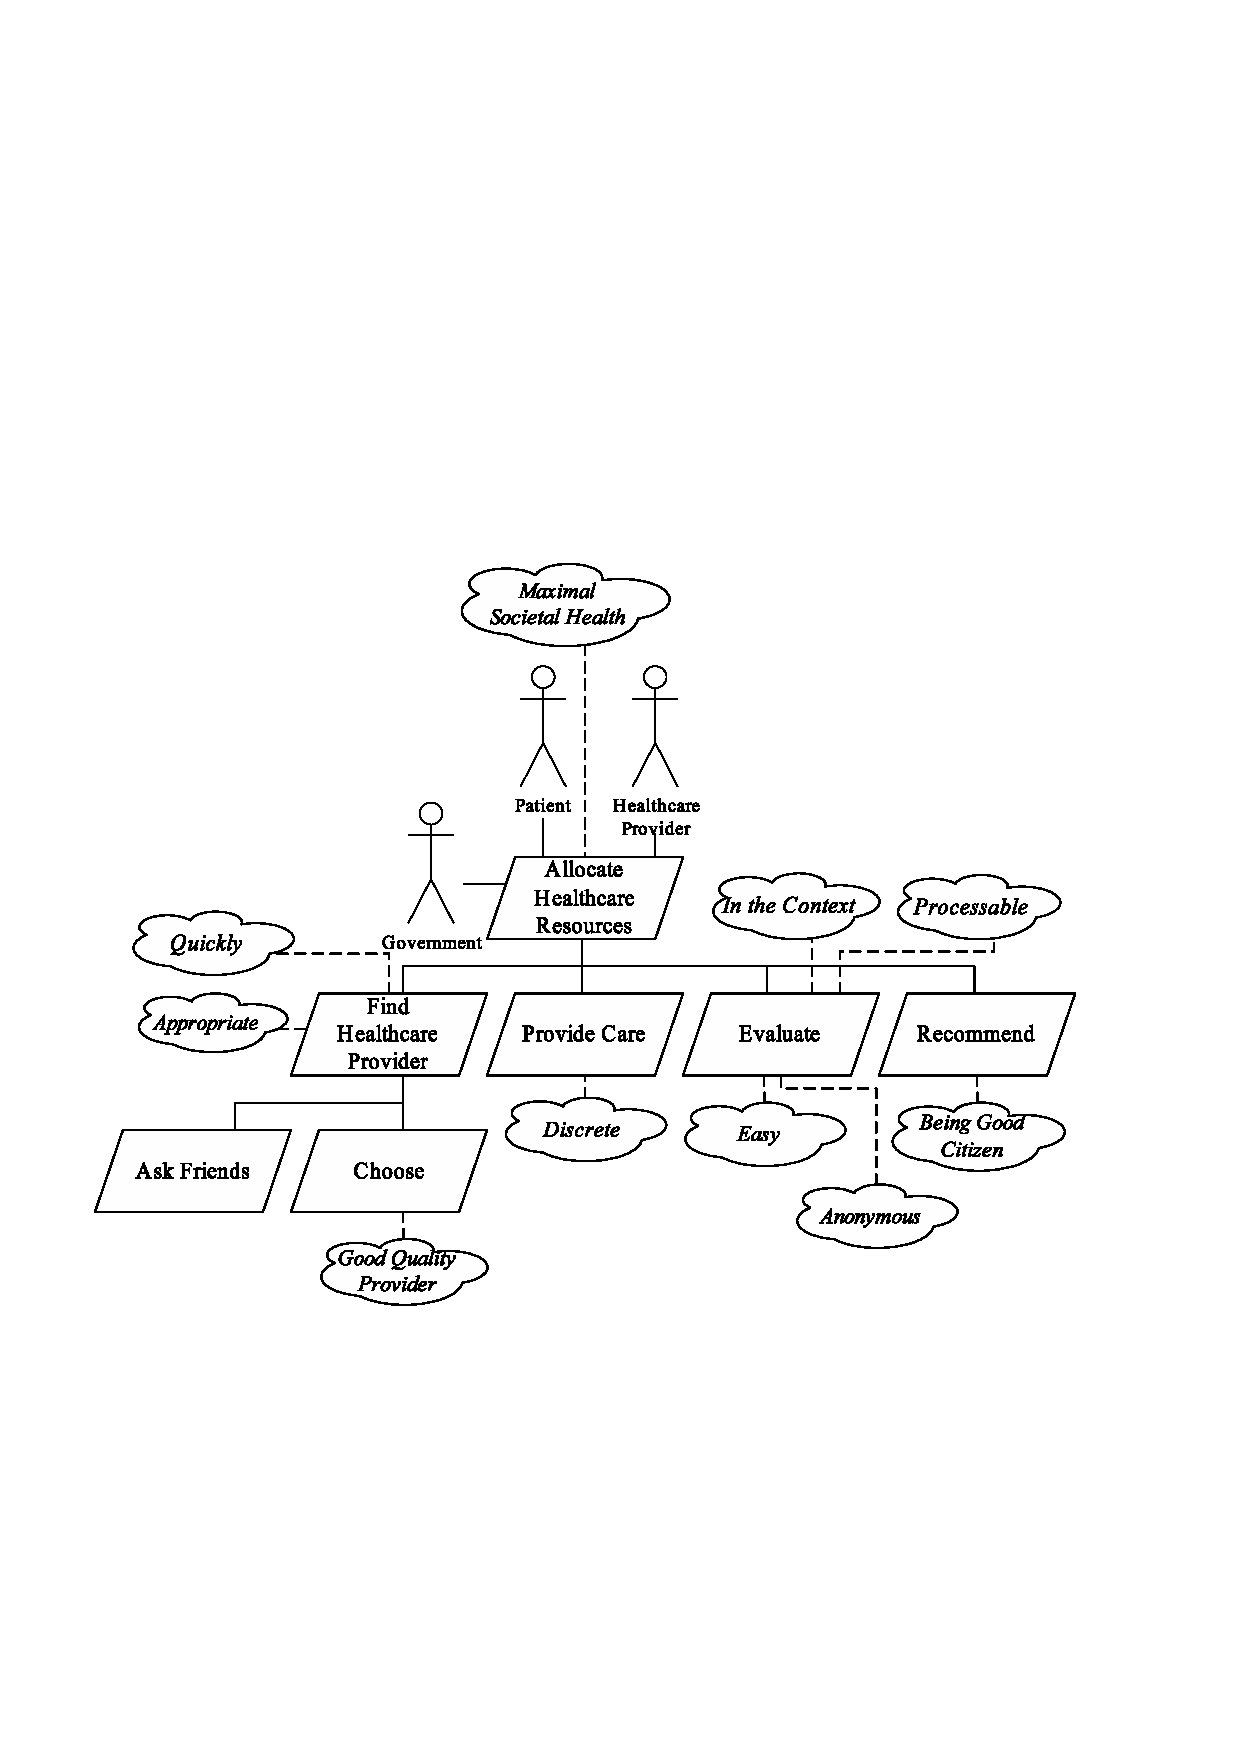
\includegraphics[scale=0.7]{chap3/chap3-fgoalmodel.pdf}
\caption{The goal model of the healthcare system}
\label{ch3:fgoalmodel}
\end{figure}

To accomplish the purpose "Allocate Healthcare Resources" of the sociotechnical system, its four subgoals need to be achieved: finding a healthcare provider, being provided with care, evaluating the care, and recommending healthcare providers to other patients. As we demonstrate below, to fulfill the goal "Find Healthcare Provider", a patient recursively asks her friends, friends' friends, and so forth for recommendations and chooses the best physician recommended. This is represented as two subgoals of "Find Healthcare Provider:" "Ask Friends" and "Choose."

We attach a number of quality goals to the functional goals in the goal model. The meanings of the quality goals are easy to understand. For example, "Quickly" means a patient wants to find a healthcare provider as soon as possible. The "Anonymous" quality goal expresses that no evaluation by a patient should identify the patient. It should be noted that the quality goal "In the Context" attached to the functional goal "Evaluate" represents that evaluation has to occur in the context of receiving the service, preferably before leaving the facilities of the healthcare provider or at least on the same day. The "Processable" quality goal means that the evaluation should be presented in a form amenable to computer processing. In our simulation, we use a scale from 1 to 5 to measure the evaluations.

According to Figure \ref{ch3:fgoalmodel}, we model two roles for our simulation - Patient and Healthcare Provider. There is also a third role - Government. Since our work focuses on the particular aspect of the U.S. healthcare domain dealing with how a patient finds a physician, rather than modeling the healthcare domain in its full complexity, the Government role's modeling is not relevant to the simulation system being designed and we ignore the Government role in our system. Additionally, we complement the goal model with the new Assistant role, which is not shown in Figure \ref{ch3:fgoalmodel}. The Assistant role is the assistant of a person and is responsible for asking friends for recommendations, choosing a healthcare provider, and assisting in evaluating the care. In the prototypical system being designed, the role of Assistant should obviously be mapped to the Assistant Agent software agent type. Since a patient is a real human that is treated by another real human - a physician - we map both the roles Patient and Healthcare Provider to the Human Agent type. The software system boundary of the sociotechnical system is obviously between the roles Patient and Assistant.

From the viewpoint of interaction analysis, the organization model of the sociotechnical system being designed is decided based on the three kinds of networks that are used for representing the relationships among the members of the society as follows. Also, we make the average degree of the three networks equal to or almost equal to a certain number, which is 6 in our case, in order to reduce the difference among different network models. The average degree of a graph is defined as $2*|E|/|V|$, where $|E|$ is the number of edges and the $|V|$ is the number of vertices in the graph.
\begin{itemize}
\item[-]Random network: the relationships between pairs of patients are created randomly until the desired number, which is 3 times of the number of nodes, to ensure the average degree is 6.
\item[-]Small-world network: most nodes are not neighbors to one another, but most nodes can be reached from any other node by a small number of hops. We followed the approach in \cite{watts1998} to construct our network by first organizing the vertices into a circle, connecting each vertex to its 3 nearest neighbors and then rewiring each edge between the vertex in question and its $k$th nearest neighbor with a 20\% probability, where $k=1, 2, 3$ for all the vertices in the graph. Edges which satisfy the condition that $k$ equals to a certain number should be rewired first and then the procedure goes on with next available $k$. The average degree is 6 in the small-world network.
\item[-]Scale-free network: the shortest paths between nodes flow through hubs, and if a peripheral node is deleted, it is unlikely that this will interfere with passing a message between other peripheral nodes. We use the Barab{\'a}si-Albert model \cite{barabasi1999} to construct a scale-free network for our simulation. Starting with two nodes, we keep adding a new node and 3 edges which connect the new node with three nodes that are already in the graph each time until we reach the desired number of nodes. For the edges, the probability of connecting with a certain node $i$ in the graph depends on the connectivity or degree of the node $k_i$ such that the probability is $k_i/\sum_{j}k_j$. For the first new node added, we add two edges because there are only two nodes in the graph in the beginning. The average degree of the scale-free network is 5.998, which is very close to 6. A scale-free network is a common model for a collaboration network.
\end{itemize}
We have shown examples of the three different networks in Figure \ref{ch3:fnetworks}. The number of persons is 15 and the average degree is 4 in these networks. The edge between two persons means they know each other.

\begin{figure}
\centering
\includegraphics[scale=1]{chap3/chap3-fnetworks.pdf}
\caption{Different networks}
\label{ch3:fnetworks}
\end{figure} 
	
After covering the viewpoints of behavior analysis and interaction analysis, we next proceed to the viewpoint of information analysis by addressing the knowledge to be represented within the system. We do this by identifying the types of knowledge entities related to the roles. As each healthcare provider has predefined capacity and efficiency, which are explained in section \ref{ch3:evaluation}, we attach the Capacity and Efficiency knowledge entity types to the Healthcare Provider role.

We now proceed to the viewpoint of interaction design. Finding a physician involves interactions between Assistant Agents representing patients. We represent these interactions as an interaction protocol between agents of the type Assistant Agent. It is appropriate to remind here that the difference between an interaction protocol and other kinds of interaction models is that an interaction protocol models some aspects of the agent behaviors along with their interactions \cite{sterling2009}.

Representing the interaction protocol of the sociotechnical system is very important, because it describes the patient's strategy of choosing a physician. We explored the following four possible choosing-a-physician strategies:
\begin{itemize}
\item[-]Random strategy. The patient's Assistant Agent randomly chooses a physician.
\item[-]The "Choose one" strategy. The patient's Assistant Agent chooses the best physician according to the patient's evaluations and his friends' evaluations. Besides the physician(s) with the best evaluation the patient already knows, his Assistant Agent asks his friends' Assistant Agents for recommendations. An Assistant Agent acting on behalf of the patient's friend may deal with the request in one of the following ways:

\begin{itemize}
\item[-]Reply with the physician(s) who has the best evaluation.
\item[-]Provide the requesting agent with the address of the Assistant Agent of one of its principal's friends if there is no recommendation to give. This process continues recursively until the first recommendation is received or until all the friends down to the maximum forwarding depth have been asked. The forwarding depth is defined as follows: the originator's friends are at depth 1; the originator's friends' friends at depth 2, and so on.
\end{itemize}

Figure \ref{ch3:fprotocol} presents the interaction protocol among patients' Assistant Agents for the "Choose one" strategy. It models that the Assistant Agent of a patient's friend may respond with a recommendation or recommend the Assistant Agent of the friend's friend. This means the interaction protocol is recursive, which is represented by the "Loop" behavioral construct. A friend's Assistant Agent may also ignore a request, which is not shown in the figure.
\end{itemize}

\begin{figure}
\centering
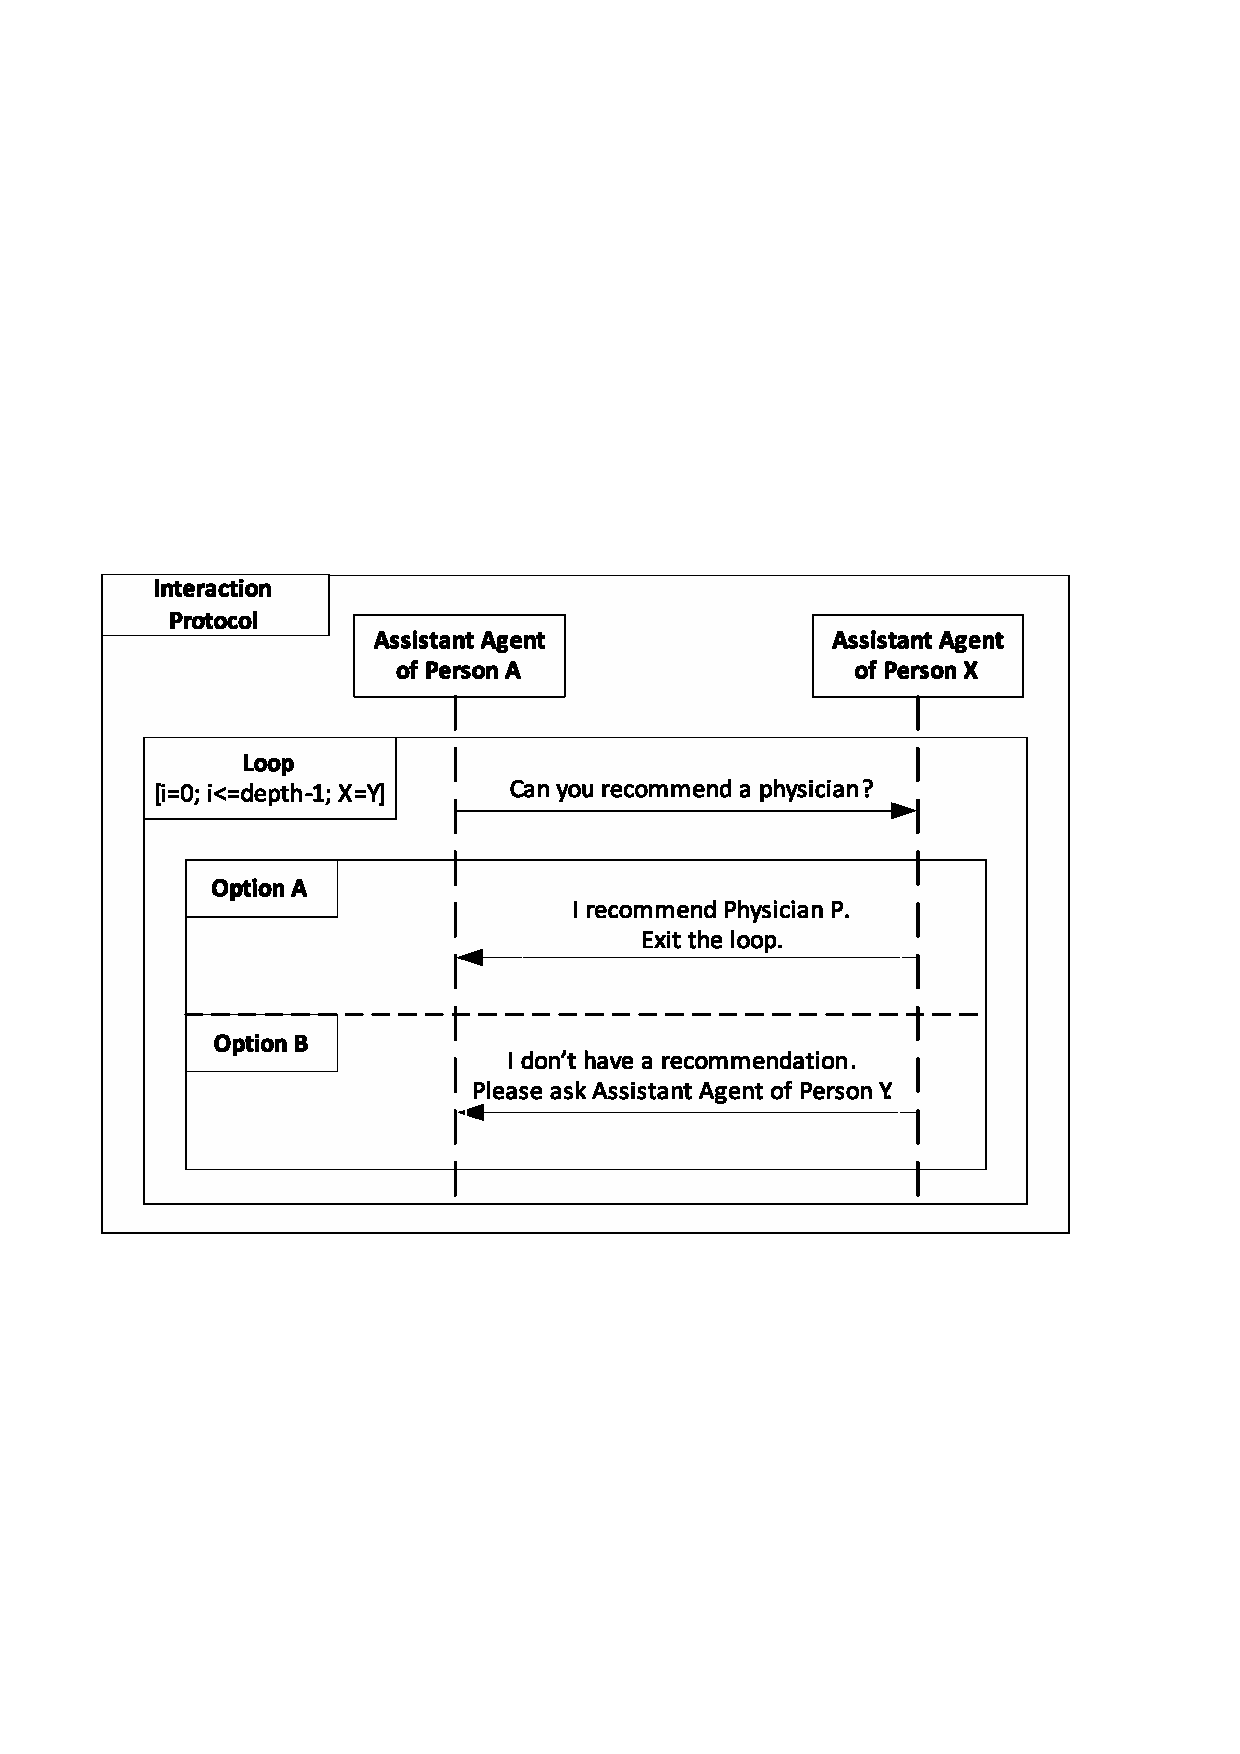
\includegraphics[scale=0.7]{chap3/chap3-fprotocol.pdf}
\caption{The interaction protocol for "Choose one" strategy}
\label{ch3:fprotocol}
\end{figure}

In addition to the random and "Choose one" strategies, we have included in our simulations the "Borda voting" and "Add and minimize" strategies. These strategies are briefly described as follows:
\begin{itemize}
\item[-]The "Borda voting" strategy. The patient's Assistant Agent asks his friends' Assistant Agents, who are closer than a specified limit in depth, for recommendations. A friend's Assistant Agent may choose to not answer, or tell the patient's Assistant Agent what it knows about all the physicians. After the patient's Assistant Agent has received all the responses, it calculates for each physician the Borda count [a single-winner election method in which voters rank candidates in order of preference, named for the 18th-century French mathematician and political scientist Jean-Charles de Borda, who devised the system in 1770], according to which a physician is given a number of points equal to the number of physicians whose evaluations are worse than the evaluations of the given physician. Thereafter the agent adds up all the points gained by the physician in question. The physician with the highest score is chosen.
\item[-]The "Add and minimize" strategy, which has the same procedure for getting recommendations as the "Borda voting" strategy. After the patient's Assistant Agent has received all the responses, it adds up all the nonzero evaluations and calculates the mean value of them for each physician. Then the Assistant Agent chooses the physician with the minimum mean evaluation. Choosing the physician with the minimum value is due to the way we define the evaluation, as described in section \ref{ch3:evaluation}.
\end{itemize}

To make it clear, Figure \ref{ch3:fchoosephysicianeg} shows an example. In the figure, a red-border box means the agent with its principle ignores the request when asked for recommendation (Allan and Erle); green means it wants to reply and it has some information (Bob, Conan, Flora and Gabby); purple means it wants to reply but it has no information (Daniel and Harris). In the "Choose one" strategy, Paul's agent asks agents of all his friends, Allan, Bob, Conan, and Daniel. Allan's agent doesn't reply for this time. Agents of Bob and Conan reply with the evaluations of the best physician(s) they know. Daniel's agent wants to reply, but it doesn't have any information. Thus, it gives Paul's agent the addresses of the agents of Daniel's friends, Gabby and Harris. Paul's agent asks Gabby's agent for recommendation and Gabby's agent replies with the best physician it knows, then Paul's agent won't ask Harris's agent any more. In the "Borda voting" and "Add and minimize" strategy, Paul's agent will ask agents of all the other persons in the figure if the depth limit is set to 2, gather evaluations of all the physicians from them and integrate these information to make a suggestion. 

\begin{figure}
\centering
\includegraphics[scale=0.7]{chap3/chap3-choosephysicianEg.pdf}
\caption{An example of different strategies}
\label{ch3:fchoosephysicianeg}
\end{figure}	
   	
From the viewpoint of behavior design, to model the behaviors of agents of the decided types, we transform responsibilities of the roles into activities attached to the agent types. As a result, we obtain behavioral scenarios for agents playing the roles Patient, Assistant, and Physician. For example, the behavioral scenario of an agent of the type Assistant Agent playing the role Assistant models that the activities "Find a physician" and "Evaluate" are performed sequentially. In a sociotechnical system for healthcare this is always the case, because the Assistant Agent does not perform any activities between these activities while a patient is attended by a physician.

Another aspect of the Assistant Agent's behavior in choosing a physician deals with what the agent should do if the physician is not available on the given day. We have decided to consider the following three waiting policies, which, for instance, could be decided by the patient's insurance company:
\begin{itemize}
\item[-]Waiting. The patient's Assistant Agent chooses the best physician by adopting one of the choosing-a-physician strategy explained above and sticks to this choice. If the physician is busy, the patient will still make an appointment with the physician and will wait until the physician becomes available.
\item[-]No waiting. If the physician chosen is busy, the patient's Assistant Agent will choose a physician randomly according to the "Random" strategy or the next best physician according to the other choosing-a-physician strategies until it finds an available physician.
\item[-]Waiting with limit. If the physician chosen is not available, the patient's Assistant Agent will check whether the physician could be reached in a certain number of days. If it is possible, the patient will make an appointment and wait. If not, the Assistant Agent will choose another physician according to the rules of the same waiting policy. If no physician is available in a certain number of days, the Assistant Agent will choose a physician who has the smallest number of days required for waiting.
\end{itemize}	
	
Finally, distinguishing between private and public knowledge entities from the viewpoint of information design is straightforward, because the knowledge entity Evaluation is private to the patient and Assistant Agent helping him/her, while the knowledge entity Recommendation is shared between different patients and instances of Assistant Agent. Similarly, the knowledge entity Efficiency is private to each Healthcare Provider, but at the same time naturally forms a basis for how patients evaluate healthcare providers. We describe models including role models, the organization model, and the domain model in detail in \cite{taveter2012}.

\section{Evaluation}
\label{ch3:evaluation}
\subsection{Simulation Settings}
We next describe from the three viewpoints introduced in section \ref{ch3:methodology} how we mapped agent-oriented models of the sociotechnical system to the programming constructs of the simulation environment.

From the viewpoint of information prototyping, we represented the knowledge entities decided by agent-oriented modeling as described in section \ref{ch3:methodology} as follows:
\begin{itemize}
\item[-]The Capacity knowledge entity - in terms of the number of patients per day that a given physician can handle.
\item[-]The Efficiency knowledge entity - in terms of the number of days that it takes for a given physician to cure a patient. This number of days is generated for each physician according to a normal distribution whose mean and standard deviation can be adjusted in the user interface.
\item[-]The Evaluation knowledge entity - in terms of the following variables:
\begin{itemize}
\item[-]The number of days the physician in question failed to handle a given patient. How this value is determined is explained below.
\item[-]The number of days that the physician needed to cure a patient. This is determined by the Efficiency knowledge item pertaining to the physician.
\item[-]A random component representing that different patients evaluate the same physician differently.
\end{itemize}
\end{itemize}
	
A patient's evaluation for a specific physician is calculated by adding these three factors. For example, let us assume that a patient gets sick today and decides to visit a physician chosen by her Assistant Agent, but the physician is busy and cannot see the patient until tomorrow. In this case, the value of the first factor - the number of days the physician in question failed to handle a given patient - is 1, because the patient had to wait for 1 day to see the physician. The second factor - the number of days that the physician requires to cure the patient - is a fixed number related to the physician in question. The third factor - the random component expressing the subjective factor - is a random value that varies between -0.5 and 0.5.

The viewpoint of behavior prototyping covers the behaviors of software agents representing patients and physicians. In accordance with the behavioral scenarios modeled as a part of the design described in section \ref{ch3:methodology}, every day the patients each try to decide which physician to visit. For each patient, the Assistant Agent acting on behalf of its principal may ask Assistant Agents of the principal's friends for recommendations and then makes a decision as to which physician the principal should visit.

From the viewpoint of interaction prototyping, the exchange of messages to be implemented is modeled according to interaction diagrams, such as the one in Figure \ref{ch3:fprotocol} for the case of choosing a physician according to the "Choose one" strategy. To make our simulations more realistic, we have chosen a 20\% probability that a friend would ignore the patient's request.

Back to the viewpoint of behavior prototyping, the software agent corresponding to the Assistant Agent recommends physicians based on evaluations. The agent can recommend only those physicians that its principal has actually visited in the simulation. The number of days the physician in question could not handle the given patient, because of the physician's exceeded capacity, accumulates in the patient's evaluation until the patient actually visits the given physician. On each new visit the agent "forgets" its previous evaluation and updates its knowledge base with the new evaluation. The reason why the agent forgets its previous evaluation is that during the time period between the previous evaluation and the new evaluation, factors that influence the evaluation may have occurred. For example, the physician may have become more skilled. Therefore it is fairer to use the latest evaluation.

To make our simulations as realistic as possible, we used the following statistical data by the Centers for Disease Control and Prevention (CDC) from the year 2008 \cite{visit}:
\begin{itemize}
\item[-]The number of physician office visits per 100 people per year: 320.1.
\item[-]The number of physicians per 10,000 people: 26.
\end{itemize}
	
Based on the above data, we obtained the average number of people who get sick every day by dividing the number of visits per 10,000 people by 250, which is the standard number of working days in a calendar year in the U.S. As a result, 128 people out of a population of 10,000 get sick every day.

\subsection{Results and Evaluation}
We simulated 365 days with 5,000 patients and 13 physicians. In our simulation, 64 random people get sick every day. The value of the local variable of each physician's software agent corresponding to the Capacity knowledge entity was set to 8 patients per day. The value of the local variable of each physician's software agent corresponding to the Efficiency knowledge entity was determined randomly according to a normal distribution with mean value 3 days and with the value of deviation as 2.0.

Figure \ref{ch3:fdays} describes the number of days needed for curing by different physicians in our simulations.

We performed simulations by combining the types of social networks with different choosing-a-physician strategies and waiting policies, which are described in section \ref{ch3:methodology}. The results from simulations in terms of the annual sick days per person and leftover patients who were not taken care of by the end of the last day simulated are represented in Tables \ref{ch3:tdran} - \ref{ch3:tpscale}.

\begin{figure}
\centering
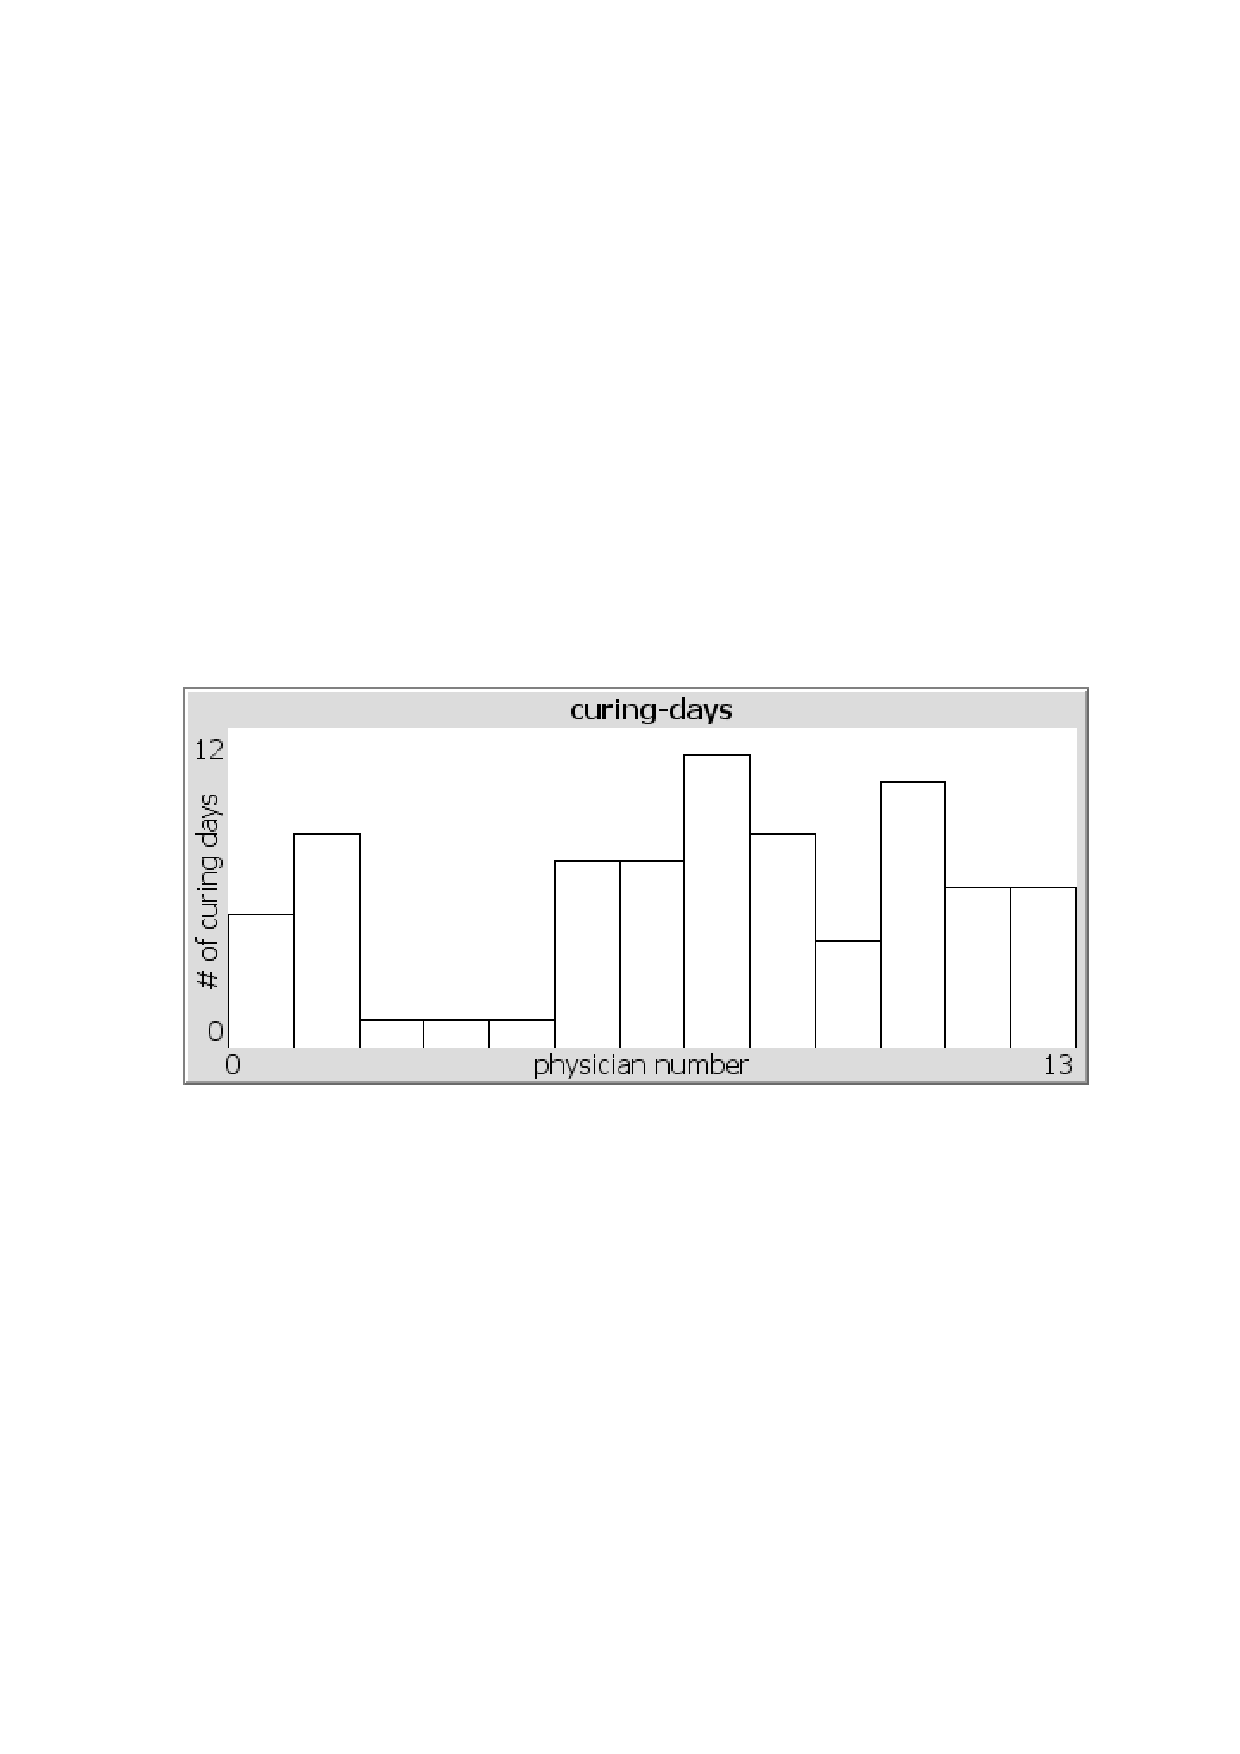
\includegraphics[scale=0.6]{chap3/chap3-fdays.pdf}
\caption{Days needed to be cured by different physicians}
\label{ch3:fdays}
\end{figure}

\begin{table}[!t]
\centering
\caption{Average sick days for random network}

\begin{tabular}{|c|c|c|c|}
\hline
& \multicolumn{3}{c|}{\textbf{Waiting policy}}\\ \hline
\textbf{Choosing-a-physician strategy}
& Waiting & No waiting & Waiting with limit\\ \hline
Random&  6.8&  6.8& 6.8\\ \hline
Choose one& 12.2 &  5.2& 6.3\\ \hline
Borda voting& 34.8 & 6.0 & 8.3\\ \hline
Add and minimize & 10.2 & 4.9 & 6.4\\ \hline
\end{tabular}
\label{ch3:tdran}
\end{table}

\begin{table}[!t]
\centering
\caption{Leftover patients for random network}

\begin{tabular}{|c|c|c|c|}
\hline
& \multicolumn{3}{c|}{\textbf{Waiting policy}}\\ \hline
\textbf{Choosing-a-physician strategy}
& Waiting & No waiting & Waiting with limit\\ \hline
Random&  0&  0& 0\\ \hline
Choose one&  427&  0& 80\\ \hline
Borda voting&  4569&  0& 96\\ \hline
Add and minimize & 155 &  0& 94 \\ \hline
\end{tabular}
\label{ch3:tpran}
\end{table}


\begin{table}[!t]
\centering
\caption{Average sick days for small-world network}

\begin{tabular}{|c|c|c|c|}
\hline
& \multicolumn{3}{c|}{\textbf{Waiting policy}}\\ \hline
\textbf{Choosing-a-physician strategy}
& Waiting & No waiting & Waiting with limit\\ \hline
Random&  6.8&  6.8& 6.8\\ \hline
Choose one& 10.3 & 5.2 & 6.3\\ \hline
Borda voting& 7.6 & 6.6 & 6.8\\ \hline
Add and minimize & 9.6 & 5.0 & 6.3\\ \hline
\end{tabular}
\label{ch3:tdsmall}
\end{table}

\begin{table}[!t]
\centering
\caption{Leftover patients for small-world network}

\begin{tabular}{|c|c|c|c|}
\hline
& \multicolumn{3}{c|}{\textbf{Waiting policy}}\\ \hline
\textbf{Choosing-a-physician strategy}
& Waiting & No waiting & Waiting with limit\\ \hline
Random& 0 & 0 & 0\\ \hline
Choose one& 407 & 0 & 71\\ \hline
Borda voting& 76 & 0 & 25\\ \hline
Add and minimize & 239 & 0 & 93\\ \hline
\end{tabular}
\label{ch3:tpsmall}
\end{table}


\begin{table}[!t]
\centering
\caption{Average sick days for scale-free network}

\begin{tabular}{|c|c|c|c|}
\hline
& \multicolumn{3}{c|}{\textbf{Waiting policy}}\\ \hline
\textbf{Choosing-a-physician strategy}
& Waiting & No waiting & Waiting with limit\\ \hline
Random& 6.8 & 6.7 &6.8 \\ \hline
Choose one& 13.7 & 5.3 & 6.3\\ \hline
Borda voting& 38.6 & 6.5 & 9.9\\ \hline
Add and minimize & 9.4 & 4.9 & 6.4 \\ \hline
\end{tabular}
\label{ch3:tdcale}
\end{table}

\begin{table}[!t]
\centering
\caption{Leftover patients for scale-free network}

\begin{tabular}{|c|c|c|c|}
\hline
& \multicolumn{3}{c|}{\textbf{Waiting policy}}\\ \hline
\textbf{Choosing-a-physician strategy}
& Waiting & No waiting & Waiting with limit\\ \hline
Random& 1 & 0 & 2\\ \hline
Choose one& 686 & 0 & 78\\ \hline
Borda voting& 4449 & 0 & 110\\ \hline
Add and minimize & 255 & 0 & 96\\ \hline
\end{tabular}
\label{ch3:tpscale}
\end{table}

We can see from Tables \ref{ch3:tdran} - \ref{ch3:tpscale} that if a patient follows the "Waiting" policy, the "Random" strategy will outperform all the other choosing-a-physician strategies in social networks of all three kinds addressed. This is the case because in all the other strategies, a patient always waits for the best physician chosen by her Assistant Agent, which increases the waiting days and accordingly sick days. Also, because the Random strategy leads to even visiting of physicians, it has no leftover patients, but there are leftover patients in the other three strategies.  

The performance of the "Borda voting" strategy is the worst in all three kinds of social networks addressed, except for the combination of the "Borda voting" strategy and "Waiting" policy in the small-world network, because it uses more evaluation information than the other strategies due to its method for calculating the votes for physicians. 

Differently from the "Borda voting" strategy, the "Add and minimize" strategy uses less information because it does not consider the physicians who have not been evaluated. The patients whose Assistant Agents follow the "Add and minimize" strategy therefore tend to choose physicians with fewer days required for curing, as compared with other choosing-a-physician strategies, and then wait for that physician chosen, which increases the number of sick days.

If the "No waiting" policy is adopted, all the other strategies will outperform the "Random" strategy. This is because the patients' Assistant Agents consider the evaluations by their principals' friends and choose the best physicians, and there is no problem of waiting.

If the "Waiting with limit" policy is adopted, the "Choose one" and "Add and minimize" strategies show the best performance. However, these strategies result in more leftover patients than the random strategy. This is reasonable, since according to "Choose one" and "Add and minimize" strategies a patient may be willing to wait for a good physician if the waiting time is less than 2 days, leading to just a few leftover patients and less average annual sick days.

According to the "Random" choosing-a-physician strategy, patients' Assistant Agents just choose physicians randomly and each physician has almost the same number of patients in total. For the other three strategies, as time passes, Assistant agents gradually gather enough information about physicians, evaluate them, and recommend to their friends the best physicians they are aware of. As a result, after patients have formed their opinions about the physicians, good physicians get full capacity of patients every day and bad physicians get only a few patients. For example, Figure \ref{ch3:ftotalnum-of-patients} shows the total number of patients going to each physician with "Waiting with limit" policy and "add and minimize" strategy in random network, and the number of patients going to each physician each day are shown in Appendix \ref{app:fhealthcarepatients}.

\begin{figure}
\centering
\includegraphics[scale=1]{chap3/chap3-fpatients.pdf}
\caption{Number of patients going to each physician in total}
\label{ch3:ftotalnum-of-patients}
\end{figure}

We also performed simulations with fewer physicians to check whether the claims stated above still hold. We adopted the "Choose one" and "Add and minimize" choosing-a-physician strategies and "No waiting" and "Waiting with limit" policies for conducting simulation experiments with 7 physicians. Table \ref{ch3:t7physician} shows the results in terms of average sick days. We can see that for the "No waiting" policy, the "Choose one" and "Add and minimize" choosing-a-physician strategies still perform better than the combination of "Random" strategy and "No waiting" policy. This is because a patient's Assistant Agent first chooses a physician who requires less days for curing and only then randomly chooses a physician if the patient has to wait.

Table \ref{ch3:t7physician} also shows that the combination of the "Waiting with limit" policy and all strategies for choosing a physician yields almost the same result.

\begin{table}[!t]
\centering
\caption{Average sick days with seven physicians}

\begin{tabular}{|c|c|c|}
\hline
& \multicolumn{2}{c|}{\textbf{Waiting policy}}\\ \hline
\textbf{Choosing-a-physician strategy}
& No waiting & Waiting with limit\\ \hline
Random& 28.0 & 19.2 \\ \hline
Choose one& 26.2 & 19.2 \\ \hline
Add and minimize & 18.3 & 19.2 \\ \hline
\end{tabular}
\label{ch3:t7physician}
\end{table}

In addition, we investigated the performance of a system having a lower probability that the friends of a patient in small-world network will answer a request, which are shown in Tables \ref{ch3:tdaysp0.6} and \ref{ch3:tdaysp0.4}. The "Random" strategy is shown here because it is not influenced by the probability.

\begin{table}[!t]
\centering
\caption{Average sick days with probability = 0.6}

\begin{tabular}{|c|c|c|c|}
\hline
& \multicolumn{3}{c|}{\textbf{Waiting policy}}\\ \hline
\textbf{Choosing-a-physician strategy}
& Waiting & No waiting & Waiting with limit\\ \hline
Choose one& 9.9 & 5.3 & 6.3\\ \hline
Borda voting& 7.6 & 6.3 & 6.6\\ \hline
Add and minimize & 9.8 & 5.0 & 6.4\\ \hline
\end{tabular}
\label{ch3:tdaysp0.6}
\end{table}

\begin{table}[!t]
\centering
\caption{Average sick days with probability = 0.4}

\begin{tabular}{|c|c|c|c|}
\hline
& \multicolumn{3}{c|}{\textbf{Waiting policy}}\\ \hline
\textbf{Choosing-a-physician strategy}
& Waiting & No waiting & Waiting with limit\\ \hline
Choose one&8.7 &5.4& 6.2\\ \hline
Borda voting&7.1& 6.1& 6.4\\ \hline
Add and minimize &10.4& 5.1 &6.4\\ \hline
\end{tabular}
\label{ch3:tdaysp0.4}
\end{table}

Comparing Table \ref{ch3:tdsmall} with these two tables, we discovered that the conclusions before still hold. To clarify this, we include Table \ref{ch3:ttrend}, which denotes the changing trend of the average sick days while the probability is decreasing. In the table, "+" means increasing and "" means decreasing. We can see from the table that for "Add and minimize", the average sick days increases while the probability decreases, because patients gets fewer responses from friends, leading to less informed decisions. For the "Borda voting" strategy, the average sick days decreases while the probability decreases. As mentioned before, due to the way that the "Borda voting" strategy gets the evaluation and calculates, it always gets too much information and lead to worse results than other strategies. So when the information is less with decreasing probability, we have better results of less average sick days. There's no fixed trend for a certain waiting policy with different choosing-a-physician strategies.

\begin{table}[!t]
\centering
\caption{Changing trend with decreasing probability}

\begin{tabular}{|c|c|c|c|}
\hline
& \multicolumn{3}{c|}{\textbf{Waiting policy}}\\ \hline
\textbf{Choosing-a-physician strategy}
& Waiting & No waiting & Waiting with limit\\ \hline
Choose one &- &+ &-\\ \hline
Borda voting &- &- &-\\ \hline
Add and minimize &+ &+ &+\\ \hline
\end{tabular}
\label{ch3:ttrend}
\end{table}

In the simulation, we don't guarantee that each patient rates all the physicians or the same number of physicians. The procedure of going to the physicians and learning about them follows a natural way in the real life if a patient asks his friends for recommendations. The patient's agent integrates the information and suggests a best physician according to a particular strategy and policy. As time goes on, everyone learns who are the best physicians and they tend to go to those physicians, so it is not the case that some patients have an undue influence on the ratings. 

If there is an epidemic in a certain area, conclusions become different for two waiting policies while the assumption of a uniform rate of sick people doesn't hold any more. In the particular area, large amount of patients rush into hospitals. If they adopt the "Waiting" policy, the patients will all be waiting for some of the physicians and it will take some patients a long time to get to the physicians except for the "Random" strategy. For the "Random" strategy, patients choose the physicians randomly and are distributed to physicians uniformly. Since the number of the patients increases a lot during epidemics, the average sick days and the number of leftover patients will definitely increase. However, our previous conclusions still hold which is the "Random" strategy will outperform other choosing-a-physician strategies. If the "No waiting" policy is adopted, patients tend to go to the best available physicians. However, because the number of the patients is too large, almost every physician will be occupied. Thus, all the choosing-a-physician strategies will perform the same as the "Random" strategy. For the same reason, if the "Waiting-with-limit" policy is adopted, all the choosing-a-physician will behave the same.

Another concern is that we only deal with general practitioners, but not specialists. If we include specialists in our system, the recommendation mechanism will work the same way as it is now. The only difference is that the ratings of specialists may probably be higher than the general practitioners. If a patient only cares about his goal, e.g., to get cured fast, without insisting choosing a specialist or a general practitioner, the system will work as before. If a patient has a request of choosing a specialist, the system could recommend him with the best specialist according to his strategy and policy with just adding a variable to indicate the type of a doctor. 
      

\section{Conclusion}
This chapter describes the design and rapid prototyping of a sociotechnical system for healthcare. Agent-oriented modeling was chosen for developing our simulation because it explicitly addresses the design of sociotechnical systems where the activities of humans are supported by software agents.

We investigated the prototyped sociotechnical healthcare system using agent-based simulations on the NetLogo platform. In the simulation, we investigated the influence of different strategies of finding an appropriate physician and different waiting policies in three common social network models. Our prototype revealed that if a patient adopts the "Waiting" policy, the "Random" strategy will outperform all the other strategies of choosing a physician. On the other hand, with the "No waiting" policy, all the other strategies will outperform the "Random" strategy. If the "Waiting with limit" policy is adopted, the "Choose one" and "Add and minimize" strategies will show the best performance. We found that by adopting the "Choose one" or "Add and minimize" strategy, in the "No waiting" and "Waiting with limit" case, the average number of sick days can be reduced by 0.4 - 1.8 days or 6\% - 27\%. If there is an epidemic, large amount of people get sick and rush into hospitals. If the "Waiting" strategy is adopted, which is rarely the case in the real world during epidemics because patients probably want to be cured as soon as possible, the "Random" choosing-a-physician strategy will outperform all the other strategies. For the other two policies, all the choosing-a-physician strategies perform the same.  

Our sociotechnical system differs from RateMDs and other similar websites where people can rate and find physicians in the way that people rate the physicians and patients interact. It is difficult to compare the effect of these websites and that of our system, mostly because there are no objective evaluation statistics on the websites, such as the length of time each patient takes to get cured during a period. Such websites use more flexible criteria on which different people might have different opinions, such as punctuality, medical knowledge, and time spent on a patient, while our system uses the time it takes to cure a patient as a criterion, which is more objective and meaningful. Although patients might access more ratings online, they usually do not know the people who have rated the physicians and there is a higher possibility that the ratings will not be truthful and accurate. In our system, a patient relies on friends' recommendations, which are typically more reliable.

Each agent in the sociotechnical system could be implemented on a mobile device which also has sensors to detect his principle's body temperature, glucose, and other health measures. In this way, the agent becomes an intelligent personal health assistant. It could warn the principle about abnormal health measures, provide suggestions on diet and exercise, and recommendations for physicians if his principle gets sick. Developing such multi-functional agents will greatly improve the life quality of people, especially those with potential health problems. 

\chapter{Determining the Effect of Personality Types on Human-Agent Interactions}
\label{ch4}

\section{Introduction}
Agents are used nowadays to help with people's everyday life in many ways. For example, an agent could help travelers find the cheapest ticket for a specific flight, or get elders their medications. Thus, it is not surprising that people have feelings about agents. It is reported that humans show empathy towards robots  \cite{lewis2013}, evidenced by measuring their emotional and neurological change when they watched videos of dinosaur robots being abused. However, people's feelings towards agents are not always positive. There's a long-existing controversy about how the agents would behave after they have too much intelligence. Some people are afraid that robots, which are a kind of agents, might kill humans if they are intelligent enough and their interests conflict with humans' interests, despite the rule of "A robot may not injure a human being or, through inaction, allow a human being to come to harm", as stated in "The Three Laws of Robotics" \cite{asimov2004robot}. Along with the technology development of many different kinds of agents, questions have risen: will humans behave preferentially towards other humans or agents? It is known that humans' personality types have impact on interactions between humans, but how about the human-agent interaction? Will a human's personality type have an impact on his/her decisions regarding other humans and agents? If we discover some relationship between personality types and decisions, how could we use these information to help with everyday life? In order to answer these questions, we must determine a human's personality type first.

\subsection{Personality Types}
There are different methods to test personality types. A famous psychometric questionnaire to reveal a person's personality type is the Myers-Briggs Type Indicator (MBTI) assessment \cite{myers1980gifts}. Myers used four dichotomies in MBTI theory, as shown in Table \ref{dich}. 

\begin{table}[!t]
\caption{MBTI Dichotomies}
\label{dich}
\centering
\begin{tabular}{|c|}
\hline
Extraversion (E) - Introversion (I)\\ \hline
Sensing (S) - iNtuition (N)\\ \hline
Thinking (T) - Feeling (F)\\ \hline
Judging (J) - Perception (P)\\ \hline
\end{tabular}
\end{table}

The result of the MBTI questionnaire is a four-letter personality type, with one letter coming from one of the four dichotomies. For example, a person with type INFP means he/she is introverted, intuitive, friendly, and more likely to probe the environment. 

We chose the Keirsey Temperament Sorter-II (KTS-II) \cite{keirsey1998please}, which is closely associated with MBTI. KTS-II classifies people into four temperament groups according to two basic dimensions of personality: what people say (communication) and what people do (action). There are two types of communication: concrete people talk about reality while abstract people talk about ideas, shown by the columns of Table \ref{kts}. Similarly, there are two types of action: cooperative and utilitarian. Cooperative people do what's right and utilitarian people do what works, as shown by the rows in Table \ref{kts}.    

\begin{table}[!t]
\caption{KTS-II dimentions}
\label{kts}
\centering
\begin{tabular}{|c|c|}
\hline
Abstract Cooperator (Idealist)& Concrete Cooperator (Guardian)\\ \hline
Abstract Utilitarian (Rational)& Concrete Utilitarian (Artisan)\\ \hline
\end{tabular}
\end{table}

The temperaments are Artisan, Guardian, Rational, Idealist, whose names come from Plato's book \emph{The Republic}. They each have different traits \cite{keirseywebsite}:
\begin{itemize}
\item[-]\textit{Idealists} speak mostly of what they hope for and imagine might be possible for people, and they want to act in good conscience, always trying to reach their goals without compromising their personal code of ethics. Examples of the Idealists are Mohandas Gandhi and Princess Diana. 
\item[-]\textit{Guardians} speak mostly of their duties and responsibilities, of what they can keep an eye on and take good care of, and they're careful to obey the laws, follow the rules, and respect the rights of others. Examples of the Guardians are George Washington and Mother Teresa.   
\item[-]\textit{Rationals} speak mostly of what new problems intrigue them and what new solutions they envision, and always pragmatic, they act as efficiently as possible to achieve their objectives, ignoring arbitrary rules and conventions if need be. Examples of the Rationals are Hillary Clinton and Stephen Hawking.
\item[-]\textit{Artisans} speak mostly about what they see right in front of them, about what they can get their hands on, and they will do whatever works, whatever gives them a quick, effective payoff, even if they have to bend the rules. Examples of the Artisans are Michael Jordan and Marilyn Monroe.
\end{itemize}

Each temperament has four variants, as shown in the first two columns in Table \ref{ktsmbti}. The third column in Table \ref{ktsmbti} shows the MBTI types corresponding to the KTS-II types. KTS-II describes behaviorial patterns while MBTI describes what people have in mind, which makes KTS-II suitable for our experiments in theory. For convenience, we sometimes use the letters from the MBTI dichotomies to denote the KTS-II personality types in this chapter.  

\begin{table}[!t]
\caption{KTS-II temperament vs MBTI type}
\label{ktsmbti}
\centering
\begin{tabular}{|c|c|c|}
\hline
\textbf{KTS-II temperament} & \textbf{KTS-II character type} & \textbf{MBTI type}\\ \hline
\multirow{4}{*}{Artisan (SP)} & Promoter&ESTP\\ \cline{2-3}
&Crafter&ISTP\\ \cline{2-3}
&Performer & ESFP\\ \cline{2-3}
&Composer & ISFP\\ \hline

\multirow{4}{*}{Guardian (SJ)} & Supervisor & ESTJ\\ \cline{2-3}
&Inspector&ISTJ\\ \cline{2-3}
&Provider & ESFJ\\ \cline{2-3}
&Protector & ISFJ\\ \hline

\multirow{4}{*}{Rational (NT)} & Fieldmarshal&ENTJ\\ \cline{2-3}
&Mastermind & INTJ\\ \cline{2-3}
&Inventor & ENTP\\ \cline{2-3}
&Architect & INTP\\ \hline

\multirow{4}{*}{Idealist (NF)} & Teacher & ENFJ\\ \cline{2-3}
&Counselor & INFJ\\ \cline{2-3}
&Champion & ENFP\\ \cline{2-3}
&Healer & INFP\\ \hline

\end{tabular}
\end{table}

\subsection{The Cake-Cutting Game}
After the human subjects get their personality types through the KTS-II test, they are asked to play the "Who Gets More Cake?" game, which is related to the classic cake-cutting game. 

In the classic cake-cutting game, players want to divide a cake in such a way that all of them believe they have received a fair amount of the cake. There are two basic measurements for a solution of the cake-cutting problem: fairness and envy-freeness. Fairness means anyone gets at least the amount that he believes is fair, while envy-freeness means anyone believes no one gets more than he has and he won't want to exchange his cake with others. If the cake is divided between two players, there is a fair and envy-free solution, which is to have one player cut the cake into two pieces and the other player choose his piece of the cake first. For three players, Selfridge-Conway discrete procedure \cite{robertson1998cake} can be used to provide a fair and envy-free solution. However, our focus here is whether humans of different personality types act differently towards an agent, not dividing the cake perfectly with fairness and envy-freeness. We add a "leftover cake giveaway" part to the cake-cutting game in our "Who Gets More Cake?" game, which will be described in detail in section \ref{ch4:exp}. 

The rest of the chapter is organized as follows. In section \ref{ch4:related}, we introduce some related work. In section \ref{ch4:exp} and \ref{ch4:results}, the experiments are described in detail and the results are analyzed. In section \ref{ch4:conclusion}, we draw the conclusion.

\section{Related Work}
\label{ch4:related}
Reeves and Nass \cite{Reeves1996} claimed that people were inclined to treat media, usually computers in their studies, as if they were real people or real places. Thus we have the hypothesis that the personality types of humans would influence their behavior towards other humans and agents, just like in the interactions between humans.

Bartneck, Hoek, Mubin, and Mahmud \cite{Bartneck2007} used "iCat" robots of different intelligent levels to test whether humans treat the robots differently. They showed that the robots' intelligence had a significant influence on the humans' decision in the measurement of their hesitation time to switch off the robot. While they investigated the influence of different intelligence levels towards humans' decision, we try to figure out whether the personality type of a human influences his decisions towards a person or an agent. 

Many researchers who investigated the influence of personality types towards humans' decisions. For example, Schmitt, Shupp, Swope, and Mayer \cite{Schmitt2008} used MBTI test to get personality types and let the human subjects play the ultimatum game. In the ultimatum game, there are two players: a proposer and a responder. The proposer first makes an offer on how to divide a given amount of money, then the responder could accept or reject. The money is divided according to the offer if the responder accepts, but none of them gets anything if the responder rejects. They discovered that the "Thinking (T)" types made lower offers than those characterized as "Feeling (F)" types and "Extraversion (E)" types indicated a willingness to accept offers that was less than "Introversion (I)" types. Peever, Johnson and Gardner \cite{Peever2012} used the Five Factor Model to test the personality types and discovered the games a person preferred was related to his personality type.

Personality traits including those in Five Factor Model \cite{digman1990} and some other traits, such as public self-consciousness and shyness are considered by Von der Putten, Kramer, and Gratch \cite{vonderputten2010}. In their study, subjects recruited through a website interacted with a virtual agent. They found that some personality traits, such as agreeableness, extraversion, approach avoidance, were related to humans' behavior, while some traits, gender, and age didn't affect the results.

We presented the questions of this chapter in the mixed human-agent society and some experimental results in \cite{du2013} \cite{du2013iat}. This chapter studies the impact of humans' personality types towards their behavior, while it is different from other studies because of three reasons: 
\begin{itemize}
\item[-]Other than MBTI or Five Factor Model, we used KTS-II test in our study, which broadens the domain of possible explanations of the influences that personality types could bring to human behavior.
\item[-]Many researchers considered the interaction between a person and an agent, sometimes just between humans, while we considered a human interacts with both a simulated human and an agent at the same time, showing the different aptitudes the human has towards the simulated human and the agent.
\item[-]We explored a different experimental setting from previous studies, which may bring new conclusions since conclusions based on previous studies might only be applied to certain studies. We developed a new game and try to figure out how humans would behave in this situation.
\end{itemize}
           


% An example of a floating figure using the graphicx package.
% Note that \label must occur AFTER (or within) \caption.
% For figures, \caption should occur after the \includegraphics.
% Note that IEEEtran v1.7 and later has special internal code that
% is designed to preserve the operation of \label within \caption
% even when the captionsoff option is in effect. However, because
% of issues like this, it may be the safest practice to put all your
% \label just after \caption rather than within \caption{}.
%
% Reminder: the "draftcls" or "draftclsnofoot", not "draft", class
% option should be used if it is desired that the figures are to be
% displayed while in draft mode.
%
%\begin{figure}[!t]
%\centering
%\includegraphics[width=2.5in]{myfigure}
% where an .eps filename suffix will be assumed under latex, 
% and a .pdf suffix will be assumed for pdflatex; or what has been declared
% via \DeclareGraphicsExtensions.
%\caption{Simulation Results}
%\label{fig_sim}
%\end{figure}

% Note that IEEE typically puts floats only at the top, even when this
% results in a large percentage of a column being occupied by floats.


% An example of a double column floating figure using two subfigures.
% (The subfig.sty package must be loaded for this to work.)
% The subfigure \label commands are set within each subfloat command, the
% \label for the overall figure must come after \caption.
% \hfil must be used as a separator to get equal spacing.
% The subfigure.sty package works much the same way, except \subfigure is
% used instead of \subfloat.
%
%\begin{figure*}[!t]
%\centerline{\subfloat[Case I]\includegraphics[width=2.5in]{subfigcase1}%
%\label{fig_first_case}}
%\hfil
%\subfloat[Case II]{\includegraphics[width=2.5in]{subfigcase2}%
%\label{fig_second_case}}}
%\caption{Simulation results}
%\label{fig_sim}
%\end{figure*}
%
% Note that often IEEE papers with subfigures do not employ subfigure
% captions (using the optional argument to \subfloat), but instead will
% reference/describe all of them (a), (b), etc., within the main caption.


% An example of a floating table. Note that, for IEEE style tables, the 
% \caption command should come BEFORE the table. Table text will default to
% \footnotesize as IEEE normally uses this smaller font for tables.
% The \label must come after \caption as always.
%
%\begin{table}[!t]
%% increase table row spacing, adjust to taste
%\renewcommand{\arraystretch}{1.3}
% if using array.sty, it might be a good idea to tweak the value of
% \extrarowheight as needed to properly center the text within the cells
%\caption{An Example of a Table}
%\label{table_example}
%\centering
%% Some packages, such as MDW tools, offer better commands for making tables
%% than the plain LaTeX2e tabular which is used here.
%\begin{tabular}{|c||c|}
%\hline
%One & Two\\
%\hline
%Three & Four\\
%\hline
%\end{tabular}
%\end{table}


% Note that IEEE does not put floats in the very first column - or typically
% anywhere on the first page for that matter. Also, in-text middle ("here")
% positioning is not used. Most IEEE journals/conferences use top floats
% exclusively. Note that, LaTeX2e, unlike IEEE journals/conferences, places
% footnotes above bottom floats. This can be corrected via the \fnbelowfloat
% command of the stfloats package.



\section{Experiment}
\label{ch4:exp}
As mentioned before, our experiment contains two phases: 
\begin{itemize}
\item[-]Test the subjects' personality types using KTS-II.
\item[-]The subjects play the "Who Gets More Cake?" game. 
\end{itemize}
Figure \ref{ch4:fmodelhai} shows the model of the human-agent interaction system. A subject shown on the left takes the personality test and plays the game with the other two players on a computer and the computer will send the result data to a database for further analysis. The upper right corner shows a simulated human who is faked by an agent. 

\begin{figure}
\centering
\includegraphics[scale=0.8]{chap4/chap4-model.pdf}
\caption{The model of the human-agent interaction system}
\label{ch4:fmodelhai}
\end{figure}

In our "Who Gets More Cake?" game, we have a cake for three players to divide. One player is the human subject/participant, one player is a simulated human, and the third player is an agent/robot (the robot has a way to convert the cake into the energy it needs to move). The participant was told he was playing with another person and a robot, but actually a simulated human and an agent for the reason of experimental control. Each player indicates how he would like to cut the cake into three pieces by drawing two lines/cuts on his own picture of the cake. Thus, we will have six lines on the cake in total after the players draw the lines. We then follow a protocol proposed by Iyer and Huhns \cite{Iyer2005}, which is proved to be fair for dividing a resource among n agents, to decide how the cake is divided: whoever has drawn the left-most cut will get the left side of the cake from the edge to this cut. Of the remaining two players, whoever has drawn the right-most cut will get the right side of the cake from this cut to the right edge. The third player will get the portion in the middle indicated by that player's two cuts. Note that all players will get one of the pieces that they indicated, as proved in  \cite{Iyer2005}. 

After the cake is divided, no player would want to trade with others, because they would get a piece that is smaller than the one they drew on the cake. However, there will be one or two portions of the cake left. To make the game more real, the participants were told one player would then be chosen randomly to give the remaining portions of the cake to one of the other players in each game. In fact, the participants were asked to whom they would give the leftover cake in every game. They could only give the leftover cake to either the simulated human or the agent, but not themselves. Each participant was asked to play the game three times, each time with a different cake and with a different simulated human. To play the part of a human as real as possible, our simulated human has different names in three games and their names are neutral to eliminate the bias of sex. At the beginning of each game, participants were asked to type a greeting sentence to the simulated human and the simulated human will type some greetings too. It takes our simulated human some time to think and draw cuts on the cake, each game with different amount of delay to mimic human thinking.

\section{Results}
\label{ch4:results}
73 non-computer science students with age around 20 who have little technological background participated in the experiment. They took the KTS-II personality test and played the game after being told the rules of the game. 58 of them played all three rounds of the game. In total, they played 197 games. We measure four criteria: 
\begin{itemize}
\item[-]The number of games in which the participants give the leftover cake to the simulated human, denoted by $N_{human}$;
\item[-]The number of games in which the participants give the leftover cake to the agent, denoted by $N_{agent}$;
\item[-]The number of participants who give the leftover cake to the same player (either the simulated human or the agent) in the three games they played, denoted by $N_{same}$;
\item[-]The number of participants who give the leftover cake to different players in the three games they played, denoted by $N_{diff}$.
\end{itemize}

The first two criteria measure the tendency that a participant would like to choose either a person or an agent under some circumstances, which might indicates whether he would like to interact with a person or an agent, and the last two criteria measure the consistency of his choice. For the last two criteria, we only consider the participants who finished all three games.
     
To deal with the personality type results, we first need to understand how to interpret KTS-II test. KTS-II provides a questionnaire based on seventy questions, each with two options indicating the two aspects of a certain dichotomy. There are ten questions for E (Extraversion)-I (Introversion) dichotomy and twenty questions each for the other three dichotomies. A personality type depends on how many options you selected for the two aspects of each dichotomy. If a person chooses the same number of options for the two aspects of any dichotomy, an "X" will appear for that dichotomy. For example, if a person choose 5 options for E (Extraversion) and 5 options for I (Introversion), his personality type will have an "X" in the E (Extraversion)-I (Introversion) dichotomy, such as XSTJ. If this happens, the person should read both ESTJ and ISTJ's descriptions and choose the one more like himself. In our experiments, a few participants have one or more "X"es in their personality types. We handle this by counting them as 1/2 person for one "X" situation for each possible type, 1/4 person for two "X"es situation for each possible type, and so on. For example, the above person with personality type XSTJ is counted as 1/2 person with type ESTJ and 1/2 person with type ISTJ.

In order to investigate how the personality types influence the choices the participants make, we introduce several statistic criteria to do evaluation: 
\begin{itemize}
\item[-]Pearson's chi-squared test ($\chi^{2}$ test) or Fisher's exact test, which evaluates the degree of independence between two nominal variables. 
\item[-]$Cram\acute{e}r's\:V\:(V)$, which is an effect size measure of association between two nominal variables.
\item[-]Goodman and Kruskal's lambda, which help us to understand whether knowing a person's personality would help to predict his choice in the game ($\lambda_{1}$) and vice versa ($\lambda_{2}$).
\end{itemize}  

\subsection{Tendency Results}
We calculated first two criteria for all the participants as a whole and have 
\begin{equation}
N_{human}=133,\:N_{agent}=64.
\end{equation} 

The data shows the participants give the leftover cake to the simulated human in most games, which is twice as many as those in which it is given to the agent. We grouped the data by sixteen MBTI types. The data is shown in Table \ref{ch4:tendencyOfMBTI}, which reveals that almost people of all the types give more leftover cakes to the humans than to the agents, which reveals their different aptitude towards the humans and the agents. Champion (ENFP), one of the Idealists, gives the leftover cakes to the simulated human 6 times than they give to the agent. On the other hand, Crafter (ISTP), one of the Artists, give more cake to the agent. $|\Delta|$ in the table is the absolute difference of $N_{human}$ and $N_{agent}$,
\begin{equation}
|\Delta|=|N_{human}-N_{agent}|.
\end{equation}
$d_r$ is the percentage difference, which is the relative difference in percentage calculated by the following formula:
\begin{equation}
d_r=\dfrac{|\Delta|}{(N_{human}+N_{agent})/2}
\end{equation}
The data is heterogeneous and it's hard to discover the pattern among all the sixteen personality types. That's one clue of suggesting us to group them in some way and analyze the results.

\begin{table}[!t]
% increase table row spacing, adjust to taste
%\renewcommand{\arraystretch}{1.3}
\caption{Tendency Results of MBTI Types}
\label{ch4:tendencyOfMBTI}
\centering
\begin{tabular}{|c|c|c|c|c|}
\hline
\textbf{MBTI type} & \boldmath{$N_{human}$} &\boldmath{$N_{agent}$} & \boldmath{$|\Delta|$} & \boldmath{$d_{r}$} \\ \hline
ESTJ	&8.25	&6.75	&1.5	&5\%	\\ \hline
ISTJ	&17.25	&9	&8.25	&16\%	\\ \hline
ESFJ	&12.875	&3.5	&9.375	&29\%	\\ \hline
ISFJ	&16.875	&7.25	&9.625	&20\%	\\ \hline
ESTP	&7	&4.5	&2.5	&11\%	\\ \hline
ISTP	&2	&2.75	&0.75	&8\%	\\ \hline
ESFP	&8.625	&3.5	&5.125	&21\%	\\ \hline
ISFP	&6.125	&2.75	&3.375	&19\%	\\ \hline
ENFJ	&3.375	&2.5	&0.875	&7\%	\\ \hline
INFJ	&5.875	&2	&3.875	&25\%	\\ \hline
ENFP	&12.625	&2	&10.625	&36\%	\\ \hline
INFP	&8.125	&5	&3.125	&12\%	\\ \hline
ENTJ	&7	&2.25	&4.75	&26\%	\\ \hline
INTJ	&8	&2.25	&5.75	&28\%	\\ \hline
ENTP	&2.25	&2	&0.25	&3\%	\\ \hline
INTP	&6.75	&6	&0.75	&3\%	\\ \hline
\end{tabular}
\end{table}


\subsubsection{KTS-II Temperaments Tendency Results}
Thus, we calculated the same criteria for the four KTS-II temperaments, as shown in Table \ref{kts1ct} and criteria for each two aspects of the four dichotomies, as shown in Table \ref{dimen1}. 

Now we want to see whether the KTS-II temperaments have significant influence on the choices the participants made. Our data fits the conditions of Pearson's $\chi^{2}$ test.  Following the test procedure, we stated the null hypothesis as follows: 

$H_{0}$: The participants' KTS-II temperaments and the choices they made are independent.

Then we represent the data in a contingency table as in Table \ref{kts1ct}, where $R_{total}$ describes row total and $C_{total}$ describes column total. The participants choices, as we observed, are called observed frequencies ($O_{freq}$) in statistics.

\begin{table}[!t]
% increase table row spacing, adjust to taste
%\renewcommand{\arraystretch}{1.3}
\caption{Observed Frequencies of Four Temperaments}
\label{kts1ct}
\centering
\begin{tabular}{|c|c|c|c|c|c|}
\hline
\boldmath{$O_{freq}$} &\textbf{Guardian} & \textbf{Artisan} &\textbf{Idealist} & \textbf{Rational} & \boldmath{$R_{total}$} \\ \hline
\boldmath{$N_{human}$} &55.25 &23.75 &30 &24 &133\\ \hline
\boldmath{$N_{agent}$} &26.5 &13.5 &11.5 &12.5 & 64\\ \hline
\boldmath{$C_{total}$} &81.75 &37.25 & 41.5 &36.5 &197\\ \hline
\end{tabular}
\end{table}

Our hypothesis is that there is no relationship between the participants' temperaments and their choices, which means they give the leftover cake to the simulated human or the agent randomly (i.e., with equal probability). Based on this hypothesis, we obtain the expected frequencies ($E_{freq}$) according to the following formula, which are the frequencies if we don't consider the factor of personality. For example, let's consider the expected frequency of $N_{human}$ for Guardian. If we don't know a person's personality, then he should give the leftover cake to the simulated human by the probability of $133/197$. With a total number of 81.75 people, the number of people who give the leftover cake to the simulated human should be $81.75*133/197=55.19$. The expected frequencies are shown in Table \ref{kts1ct2}.
\begin{equation}
E_{freq}=C_{total}*R_{total}/T
\end{equation}
For a specific cell in the expected frequency table, $C_{total}$ in the above formula is the column total for the column of that cell, while $R_{total}$ is the row total for the column of that cell. $T$ in the formula is the number of games played in total, which is 197 in our case. 

\begin{table}[!t]
% increase table row spacing, adjust to taste
%\renewcommand{\arraystretch}{1.3}
\caption{Expected Frequencies of Four Temperaments}
\label{kts1ct2}
\centering
\begin{tabular}{|c|c|c|c|c|}
\hline
\boldmath{$E_{freq}$} &\textbf{Guardian} & \textbf{Artisan} &\textbf{Idealist} & \textbf{Rational} \\ \hline
\boldmath{$N_{human}$} &55.19 &25.15 &28.02 &24.64 \\ \hline
\boldmath{$N_{agent}$} &26.56 &12.10 &13.48 &11.86 \\ \hline
\end{tabular}
\end{table}

We use the following formula to calculate $\chi^{2}$:
\begin{equation}
\chi^{2}=\sum_{0<i<m,\:0<j<n}
\frac{(O_{freq}(i,j)-E_{freq}(i,j))^{2}}{E_{freq}(i,j)},
\end{equation}
where $O_{freq}(i,j)$ and $E_{freq}(i,j)$ denote the observed frequencies and expected frequencies in the table cell of $i$th row and $j$th column. $m$ and $n$ represents the total row number and total column number. The statistical results are  
\begin{equation}
\chi^{2}=0.72,\:P=0.87,\:V=0.06.
\end{equation}
$P$ is one-tailed (right-tail) probability value for a chi-square test (i.e., the area under the chi-square distribution from the chi-square value to positive infinity), given the chi-square value and the degree of freedom, which can be calculated through a lookup table or an online tool. The degree of freedom $df$ is the number of values in the table that are free to vary given existing constrains. In our table, $R_{total}$ and $C_{total}$ are the constrains fixed for each row and column. In the table, we only need to vary the contents of 3 cells and the contents of the rest cells could be decided then. Thus, the degree of freedom is 3 in our case. $V$ is calculated using the following formula:
\begin{equation}
\sqrt{\frac{\chi^{2}}{T*(k-1)}},
\end{equation}
where $T=197$ and $k=2$, which is the smaller number of the number of rows and the number of columns in the table. 

The meaning of the result is that we are $1-P$ (in the form of percentage) sure to reject the null hypothesis. Normally significant level of 0.05 or 0.1 is used, which means if $P<0.05$ or $P<0.1$ we can reject the hypothesis. In our case, $P>0.05$ and there is 13\% probability that we could reject the hypothesis, which is very low. Thus we can't reject the null hypothesis, which means we can't say there is a relationship between the participants' temperaments and their choices. $V$ is an effect size measure which shows the inter-correlation of the variables. In this case, it measures the relationship between the participants' KTS-II temperaments with their choices. According to the convention, $V<0.1$ means negligible relationship. In our case, $V=0.06$ means the association between the KTS-II temperaments and the choices is negligible.   

Percentage deviation, which measures the degree to which observed frequencies differs from the expected frequencies, is calculated as follows:
\begin{equation}
PD(i,j)=\frac{O_{freq}(i,j)-E_{freq}(i,j)}{E_{freq}(i,j)}.
\end{equation}

Table \ref{kts1pd} shows the percentage deviation of the KTS-II temperaments' tendency results, from which we could see that people with different temperaments behave very differently. Artisans and Idealists are deviated more from the general public than the other two temperaments. The Guardians act just like an average person. By an average person, we refer to an imaginary person who will act as our reference data shows. For example, if this person plays our game for 197 times, he would probably end up with giving the leftover cake 133 times to the simulated human and 64 times to the agent.

\begin{table}[!t]
% increase table row spacing, adjust to taste
%\renewcommand{\arraystretch}{1.3}
\caption{Percentage Deviation of Four Temperaments}
\label{kts1pd}
\centering
\begin{tabular}{|c|c|c|c|c|}
\hline
\textbf{Percentage Deviation} &\textbf{Guardian} & \textbf{Artisan} &\textbf{Idealist} & \textbf{Rational} \\ \hline
\boldmath{$N_{human}$} &0.1\% &-5.6\% &7.1\% &-2.6\% \\ \hline
\boldmath{$N_{agent}$} &-0.2\% &11.6\% &-14.7\% &5.4\% \\ \hline
\end{tabular}
\end{table}

At last we use Goodman and Kruskal's lambda to measure the proportional reduction in error. For example, in our case, the estimated probability of correct prediction when predicting a person's choice without knowing his temperament is 
\begin{equation}
p_{1}=\frac{133}{197}=0.68,
\end{equation}
while estimated probability of correct prediction when predicting what choice a person will make knowing his temperament is
\begin{equation}
p_{2}=\frac{55.25+23.75+30+24}{197}=0.68.
\end{equation}
Goodman and Kruskal's lambda of predicting choice on the basis of temperament is 
\begin{equation}
\lambda_{1}=\frac{(1-p_{1})-(1-p_{2})}{1-p_{1}}=0,
\end{equation} 
which means there is no difference whether or not knowing a person's temperament when predicting his choice. Also we found out lambda of predicting a person's temperament from his choice ($\lambda_{2}$), which is calculated according to a similar way as that of $\lambda_{1}$, is 0, meaning knowing a person's choice won't do any good to predicting the his temperament.       

To give a hint of how the participants' choices of each dichotomy varies, table \ref{dimen1} shows the tendency results of four dichotomies, where $PD_{human}$ is the percentage deviation of $N_{human}$ and $PD_{agent}$ is the percentage deviation of $N_{agent}$. We could see that the biggest difference from what is supposed to be with our equal probability assumption happens in the T-F dichotomy.

\begin{table}[!t]
% increase table row spacing, adjust to taste
%\renewcommand{\arraystretch}{1.3}
\caption{Tendency Results and Percentage Deviation of Four Dichotomies}
\label{dimen1}
\centering
\begin{tabular}{|c|c|c|c|c|}
\hline

\textbf{MBTI dichotomy} & \boldmath{$N_{human}$} &\boldmath{$N_{agent}$} & \boldmath{$PD_{human}$} & \boldmath{$PD_{agent}$} \\ \hline
E (Extraversion)&	62&	27 &3.2\% &-6.6\%\\ \hline
I (Introversion)&	71&	37 &-2.6\% &5.5\%\\ \hline
S (Sensing)&	79&	40 &-1.7\% &3.5\% \\ \hline
N (iNtuition)&	54&	24 &2.5\% &-5.3\% \\ \hline
T (Thinking)&	58.5&	35.5 &-7.8\% &16.2\% \\ \hline
F (Feeling)&	74.5&	28.5 &7.1\% & -14.8\%\\ \hline
J (Judging)&	79.5&	35.5 &2.4\% & -5.0\%\\ \hline
P (Perception)&	53.5&	28.5 &-3.4\% & 7.0\% \\ \hline
\end{tabular}
\end{table}

Then we investigated how MBTI dichotomies influence the choices the participants made. Following the same procedure, first we stated the null hypothesis for each dichotomy as follows:
\begin{itemize}
\item[-]For E-I dichotomy: The participants' types in E-I dichotomy and their choices are independent;
\item[-]For S-N dichotomy: The participants' types in S-N dichotomy and their choices are independent;
\item[-]For T-F dichotomy: The participants' types in T-F dichotomy and their choices are independent;
\item[-]For J-P dichotomy: The participants' types in J-P dichotomy and their choices are independent.
\end{itemize} 

Table \ref{dimen1results} shows the statistic results for each dichotomy. From the table we could see that in T-F dichotomy, there is 87\% possibility, which is close to the standard of rejecting the null hypothesis with a significance level of 0.1, to reject the null hypothesis. Still, we can't reject the null hypothesis, but we probably could see it get rejected with more experiments and draw a conclusion that the personality in T-F dimension has something to do with the participants' choices based on statistics. For other dimensions, there is no evidence to lead to the conclusion that we should reject the null hypothesis and say there is a relationship between a certain dichotomy and the choices. 

Also, we could see from $Cram\acute{e}r's\:V$ there's a weak relationship between T-F dichotomy and the choices, and negligible relationship between any other dichotomy and the choices in the whole population based on our samples. $\lambda_{2}$ for T-F dichotomy is 0.07, which means that we could reduce 7\% error when predicting a person's temperament with his choice known compared to that with his choice not known.     

\begin{table}[!t]
% increase table row spacing, adjust to taste
%\renewcommand{\arraystretch}{1.3}
\caption{Statistical Results of Four Dichotomies for Tendency}
\label{dimen1results}
\centering
\begin{tabular}{|c|c|c|c|c|c|}
\hline
\textbf{MBTI Dichotomy} &\boldmath{$\chi^{2}$} & \boldmath{$P$} &\boldmath{$V$} & \boldmath{$\lambda_{1}$} & \boldmath{$\lambda_{2}$} \\ \hline
E-I &0.34 &0.56 &0.04 &0 &0\\ \hline
S-N &0.17 &0.68 &0.03 & 0 &0 \\ \hline
T-F &2.28 &0.13 &0.11 & 0 & 0.07\\ \hline
J-P &0.33 &0.57 &0.04 &0 &0 \\ \hline
\end{tabular}
\end{table}


\subsection{Consistency Results}
Next, we measure the consistency of the participants' choices. First we calculated the consistency criteria:
\begin{equation}
N_{same}=18,\:N_{diff}=40.
\end{equation} 
We could see that more than two thirds of participants give the leftover cake to different players in three games, which means they don't always prefer the simulated human or the agent. Similar to the tendency results, we grouped the $N_{diff}$ and $N_{same}$ data according to temperaments and dichotomies, shown in the first three columns in Table \ref{kts2} and Table \ref{dimen2}. We could consider the consistency as "fairness" in the sense that the participants try to behave "fairly" by giving the leftover cake to the simulated human and the agent in three repetitions of the game, rather than to only one of them.    

It is not suggested to use Pearson's $\chi^{2}$ test if there are small expected frequency values, so we use Fisher's exact test here to perform analysis similar to Pearson's $\chi^{2}$ test for data in Table \ref{kts2} and it turns out $P$ is very close to 1. We also perform Pearson's $\chi^{2}$ test to get an approximate $V$ value. Our null hypothesis is as follows: 

$H_{0}$: The participants' KTS-II temperaments and the consistency results of their choices are independent.

The statistical results are as follows:
\begin{equation}
\chi^{2}=0.22,\:V=0.06,\:\lambda_{1}=0,\:\lambda_{2}=0.
\end{equation}
It shows that there is no significant dependence between the participants' KTS-II temperaments and the consistency of their choices. A person's temperament has little association with the consistency of his choices. Knowing a person's temperament or the consistency of his choices won't do any help to the prediction of the consistency of his choices or his temperament.

\begin{table}[!t]
% increase table row spacing, adjust to taste
%\renewcommand{\arraystretch}{1.3}
\caption{Consistency Results and Percentage Deviation of Four Temperaments}
\label{kts2}
\centering
\begin{tabular}{|c|c|c|c|c|}
\hline
\textbf{KTS-II Temperament}& \boldmath{$N_{same}$} & \boldmath{$N_{diff}$} & \boldmath{$PD_{same}$} & \boldmath{$PD_{diff}$}\\ \hline
Guardian& 7.75&	16.5 & 3.0\% & -1.3\%\\ \hline
Artisan& 3.25&	7.5 & -2.6\% & 1.2\% \\ \hline
Idealist& 3&	8.5 &-15.9\% &7.2\%\\ \hline
Rational& 4&	7.5 &12.1\% &-5.4\% \\ \hline
\end{tabular}
\end{table}

Then we investigated how MBTI dichotomies influence the consistency of the choices that the participants made. Following the same procedure, first we stated the null hypothesis for each dichotomy as follows:
\begin{itemize}
\item[-]For E-I dichotomy: The participants' types in E-I dichotomy and the consistency of their choices are independent;
\item[-]For S-N dichotomy: The participants' types in S-N dichotomy and the consistency of their choices are independent;
\item[-]For T-F dichotomy: The participants' types in T-F dichotomy and the consistency of their choices are independent;
\item[-]For J-P dichotomy: The participants' types in J-P dichotomy and the consistency of their choices are independent.
\end{itemize} 

\begin{table}[!t]
% increase table row spacing, adjust to taste
%\renewcommand{\arraystretch}{1.3}
\caption{Consistency Results and Percentage Deviation of Four Dichotomies}
\label{dimen2}
\centering
\begin{tabular}{|c|c|c|c|c|}
\hline
\textbf{MBTI dichotomy} & \boldmath{$N_{same}$} & \boldmath{$N_{diff}$} & \boldmath{$PD_{same}$} & \boldmath{$PD_{diff}$}\\ \hline
E (Extraversion)&	9&	15.5 &18.4\% &-8.3\%\\ \hline
I (Introversion)&	9&	24.5 &-13.4\% &6.0\%\\ \hline
S (Sensing)&	11&	24 & 1.3\% & -0.6\%\\ \hline
N (iNtuition)&	7&	16 & -1.9\% &0.9\%\\ \hline
T (Thinking)&	8.5&	20 &-3.9\% &1.8\%\\ \hline
F (Feeling)&	9.5&	20 & 3.8\% &-1.7\%\\ \hline
J (Judging)&	11.5&	22 &10.6\% &-4.8\%\\ \hline
P (Perception)&	6.5 &18 &-14.5\% &6.5\%\\ \hline
\end{tabular}
\end{table}

\begin{table}[!t]
% increase table row spacing, adjust to taste
%\renewcommand{\arraystretch}{1.3}
\caption{Statistical Results of Four Dichotomies for Consistency}
\label{dimen2results}
\centering
\begin{tabular}{|c|c|c|c|c|c|}
\hline
\textbf{MBTI Dichotomy} &\boldmath{$\chi^{2}$} & \boldmath{$P$} &\boldmath{$V$} & \boldmath{$\lambda_{1}$} & \boldmath{$\lambda_{2}$} \\ \hline
E-I & 0.64 & 0.42 & 0.11 & 0 & 0\\ \hline
S-N & 0.01 & 0.92 & 0.01 & 0 & 0\\ \hline
T-F &0.04 & 0.84 & 0.03 & 0 & 0\\ \hline
J-P & 0.4 & 0.53 & 0.08 & 0 & 0\\ \hline
\end{tabular}
\end{table}

Table \ref{dimen2}, where $PD_{same}$ and $PD_{diff}$ denote the percentage deviation of $N_{same}$ and $N_{diff}$, gives us a hint of how the observed data deviates from what should be with equal possibility assumption. E-I and J-P dichotomies deviates more than the other two dichotomies. The statistical results are shown in Table \ref{dimen2results}, based on which we couldn't reject any of the null hypothesis and say any dichotomy and the consistency results are not independent. Besides, knowing a person's dichotomies or the consistency of his choices won't do any help to the prediction of the consistency of his choices or dichotomies. However, $Cram\acute{e}r's\:V$ shows there is a weak association between E-I dichotomy and the consistency of the choices. In conclusion, being fair is more important than personality.  
 

\section{Conclusion}
\label{ch4:conclusion}
In this chapter, we try to investigate whether humans' behavior towards other humans and agents is related to their personality types. We have seventy-three students participated in the experiments, by taking the KTS-II test and then playing the "Who Gets More Cake?" game. 

We discovered that humans of different personality types behave differently towards other humans and agents. For example, Artisans and Idealists act more deviated from an average person; it's very likely that T-F dichotomy is not independent with the tendency results. This provides a clue in many agent-related applications. For example, an Idealist has to partner
with an agent/robot as his personal assistant due to business
reasons. As an Idealist, he is inclined to interact with humans more and agents less, thus he might choose an robot with less talking
or interactions needed. In the next stage, we may discover agents of which personality type could cooperate well with a certain kind of person, which could be used in many domains, such as elder's personal care, team formation and so on. 

Currently our experiments shows little clue of making predictions based on a person's personality. In the future, we expect that more students participate in an updated version of this experiment to draw more reliable conclusion based on our statistical criteria and explore other possibilities. Also, the personality types of the simulated human and the agent are not considered yet. We expect to find a way to integrate this factor into the future experiments.  

% ********** Chapter 6 **********
\chapter{Conclusion}
\label{ch5-conclusion}

Agents are involved in humans' everyday life and thus humans with the help of agent technologies form different sociotechnical systems under various situations. The reason why humans need technical help is the increasing complexity of ongoing problems in the society. For the complex problems that are beyond the ability of individuals, it is promising to take advantage of advanced technologies to cope with them. For technical help, we consider two aspects, which are how to represent and use the interactions of agents acting on behalf of humans, and how a person interacts with the system or the agent. In this dissertation, we investigated these two aspects by studying three cases using the case study approach.

The first case is a multiagent shopping system that could give a customer suggestions on where to shop and what to shop. We proposed an approach, tested it with simulated price data and real price data collected from nearby stores, and compared it with three other common approaches. It is shown that at least 22\% savings could be made generally with simulated data. With the real data, a customer could save 6\% more using our approach. We also proved robustness of our approach under the situation of deceptive stores with simulated data and wrongly reported price with real data.  
 
The second case is a multiagent healthcare system in which agents representing patients could exchange information about physicians and recommend the most proper physician to a patient. We considered three kinds of networks: random network, scale-free network, and small-world network to represent the social relationship of people. We assume that if two people know each other, their agents know each other too. The agent of a patient asks the agents of the patient's friends for information about physicians they know. Depending on different choosing-a-physician strategies and waiting policies, the patient may get different recommendations of a physician. As for the number of annual sick days per person in different situations, it is shown that 0.4-1.8 days could be reduced using the sociotechnical system compare to that of choosing a physician randomly. 

In the third case, we are trying to investigate a factor, personality to be particular, that influences human-agent interaction. To achieve this purpose, we test human subjects' personality and have them play the "Who Gets More Cake?" game. The game is designed in such a way that at the end of the game each subject is asked a question that indicates his inclination towards humans or agents. The result shows that humans treat other humans and agents differently and humans with different personalities behave differently. However, fair is more important than personality types, which means the subjects would try to treat humans and agents differently, but in the same extent of difference regardless of their personalities.     

Agents are involved in the sociotechnical systems in all three cases. In the grocery shopping case, agents work together indirectly through the central manager of the online system. If we could scan the items and the information related to the items could be taken and uploaded by an agent possibly installed on our cellphone automatically to the online system, people could save a lot of money by sharing the information they know. In the healthcare case, agents communicate and collect more information than that could be collected by only one person and utilize integrated information to give suggestions. In the human-agent interaction case, humans' reaction to other humans and agents are observed and the effect of personality as a factor is investigated. Through the three cases, it is shown that agents, which could be considered as a piece of autonomous intelligent software, could provide suggestions to humans by integrating information that a human could not or does not willing to handle. Along with the rapid development of technologies and thus huge amount of information, the need of agents in different areas of human life is growing bigger and bigger. Thus, we foresee that agent technologies will be widely used in the future than it is today.

However, there are limitations in our case studies. For the shopping system, we need some way to get the item information automatically to the online system, which might be difficult because stores may not want to provide the convenience of getting item information they have already stored in their system by simply letting customers scan the barcode.

For the healthcare system, real life is much more complex than our simulation. First, we simplify the question by making the patients and physicians homogeneous, that is, each person behaves similarly to the other persons of the same kind. For example, the ratings of a physician from different patients won't vary too much; each physician could take care of the same number of patients at most every day; the number of patients distributed evenly throughout the year, etc. We assume that patients all adopt the same choosing-a-physician strategy and waiting policy in a particular simulation, which is not true in the real world since everyone might have different preferences over these choices and each person may have different preferences depending on the severity of his disease. Second, we didn't consider unforeseen situations or the variables. For example, a patient may change his/her idea in the middle of the treatment, such as switching to another physician if he/she is not satisfied with the current physician.  

In the human-agent interaction case, there might be multiple factors that influence humans' decisions in the game. We didn't consider the interactions of different factors and actually it's even impossible to list all the factors. Also, the subjects in our experiment are students around 20s. If we want to generalize the conclusion, we need to collect data from more subjects of various ages, educational background and so on. In this way, we could get more useful and accurate conclusion. Moreover, if we have large amount of subjects of different background play different games, we might find some pattern that could guide us and learn more about the effects of personality or other factors on humans' attitude towards other humans and agents.

Based on our experience, here are some recommendations for designing sociotechnical systems:
\begin{itemize}
\item[-]Model the problem as realistically as possible. When designing a sociotechnical system for research purposes, simplifications are usually made because it is difficult to make it just like in a complex real life situation. However, it is necessary to model the problem in question complex enough to make sure it doesn't lack of any critical factors that might influence the conclusion. 
\item[-]Carefully design the rules of the interaction among agents, and the interaction between a human and an agent. Different systems may require different rules of interaction, so it is important to define the norms and have all the agents follow the norms.   
\item[-]Consider possible variables in the system and perform a robustness analysis. In most systems, there are variables that may change at some point or wrong data input depending on the designed system. These uncertainties should be considered and taken care of.
\end{itemize}

To summarize, agent technologies can have important effect on aiding or facilitating humans' everyday life in various kinds of sociotechnical systems. To better accomplish this purpose, we need to understand how the agents could help in sociotechnical systems, which motivates this dissertation. There are additioanl studies that could be done to improve the work in this dissertation. For the shopping suggestion system, a mobile app could be developed and used to upload the information to the central manager; real shopping lists of different types of families could be used to further test the system. For the healthcare system, a more complex model is needed to overcome the shortcomings mentioned in the limitations part. For the human-agent interaction case, more subjects of different background could be very helpful to draw a more accurate conclusion. Exploring different possibilities of improving these case studies could help us to understand aspects of implementing sociotechnical systems more in depth, thus providing useful tools for assisting humans with complex problems that are hard to cope with.             


%\include{Conclusion}     %% Honors theses are required to 
                          %% have an unnumbered chapter
                          %% for conclusions.  The file
                          %% Conclusion.tex should begin
                          %%   
                          %% \chapter*{Conclusion}
                          %% followed by the appropriate
                          %% text.

\include{biblio}            %% The calls the file biblio.tex
                          %% The contents of this file depend
                          %% on how you have chosen to do
                          %% your bibliography. 

\Appendix                 %% Use this command if you have one 
                          %% appendix. Use \Appendices if you 
                          %% have more than one.
	
% ********** Appendix A **********

\chapter{Item Prices in Dollars}
\label{app-table1}
\includepdf[pagecommand={\thispagestyle{plain}},pages={1},scale=1]{appendices/shoppingdata.pdf}

%\begin{table}[!t]
 % \caption{Item Prices in Dollars}
  %\centering
  %\begin{tabular}{c}
%\begin{center}                                                                         
   %   \includegraphics[width=0.9\textwidth]{appendices/shoppingdata.pdf} 
 %   \end{center}     
 % \end{tabular}
%\end{table}
% ********** End of appendix **********         %% Calls toolong.tex which contains
\chapter{Number of patients going to each physician each day}
\label{app:fhealthcarepatients}
\includepdf[pagecommand={\thispagestyle{plain}},pages=-,scale=1]{appendices/patients.pdf}

%\begin{figure}
%\centering
%\includegraphics[scale=1,page=1]{appendices/patientsPage4.pdf}
%\caption{Number of patients going to each physician each day}
%\end{figure}
                          %% an appendix. After issuing the 
                        %% command \Appendix or \Appendices
                        %% you must use \input not \include
                        %% to load the first appendix.

\end{document}
%%%%%%%%%%%%%%%%%%%%%%%%%%%%%%%%%%%%%%%%%%%%%%%%%%%%%%%%%%%%%%%
